\documentclass[a4paper,titlepage,12 pt,twoside]{report}
\usepackage[bindingoffset=1cm,centering,includeheadfoot,margin=3cm]{geometry}
\usepackage[T1]{fontenc}
\usepackage[latin1]{inputenc}
\usepackage[english,italian]{babel}


\usepackage{lipsum}                        % testo fittizio
%immagini
\usepackage{graphicx}
%gruppi di immagini
\usepackage{subfig}
%formule matematiche display
\usepackage{amsmath}
\usepackage{amssymb}
%linee tabelle
\usepackage{booktabs}
%bibliografia
\usepackage[autostyle,italian=guillemets]{csquotes}
\usepackage[style=numeric-comp, backend=biber]{biblatex}
\addbibresource{bibliografia.bib}
%codice sorgente
\usepackage{listings}
\usepackage{xcolor}
\definecolor{mygreen}{rgb}{0,0.6,0}
\definecolor{mygray}{rgb}{0.5,0.5,0.5}
\definecolor{mymauve}{rgb}{0.58,0,0.82}

\lstdefinestyle{signature}{
basicstyle=\small\ttfamily,
language=C,
numbers=none,
numberstyle=\tiny,
breaklines=true,
literate = {\\-}{}{0\discretionary{-}{}{}},
showstringspaces = false
}

\lstdefinestyle{input}{
frame = single,
basicstyle=\ttfamily\scriptsize,
language=C,
numbers=left,
numberstyle=\tiny,
breaklines=true,
captionpos=b,
commentstyle=\color{mygreen},
keywordstyle=\color{blue},   
stringstyle=\color{mymauve},
showstringspaces = false
}

\lstset{
basicstyle=\small\ttfamily,
language=C,
numbers=left,
numberstyle=\tiny,
breaklines=true,
captionpos=b,
commentstyle=\color{mygreen},
keywordstyle=\color{blue},   
stringstyle=\color{mymauve},
literate = {\\-}{}{0\discretionary{-}{}{}},
showstringspaces = false}
\addto\captionsitalian{
\renewcommand{\lstlistingname}{Codice}}
\addto\captionsitalian{
\renewcommand{\lstlistlistingname}{Elenco dei codici}}
%collegamenti ipertestuali
\usepackage{hyperref}
\hypersetup{hidelinks}
%testatine
\pagestyle{headings}
%commenti
\usepackage{comment}
%grafici
\usepackage{pgfplots}
\usepackage{tikz}
\pgfplotsset{/pgf/number format/use comma,compat=newest}


\begin{document}

\newcommand{\HRule}{\noindent\rule{\linewidth}{0.3mm}}

\begin{titlepage}
\begin{center}

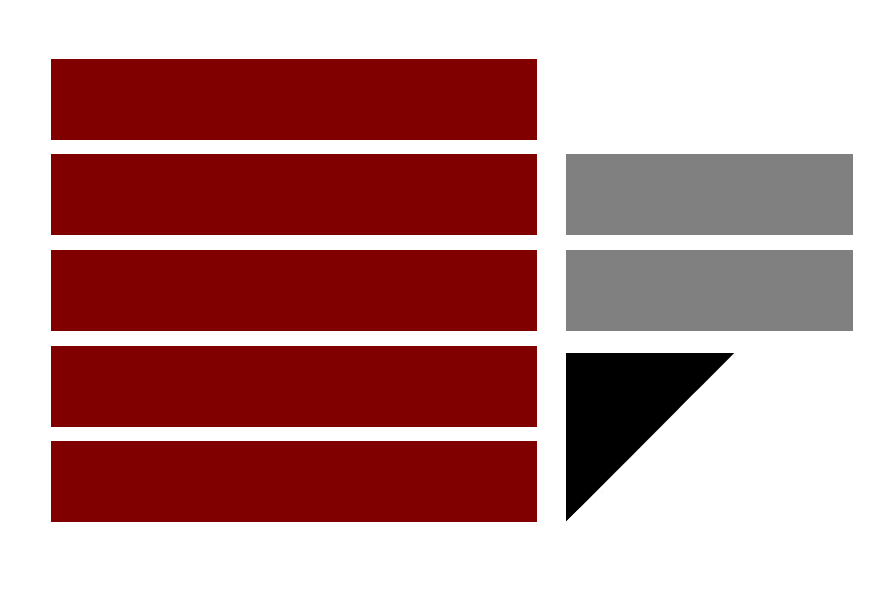
\includegraphics[width=0.35\textwidth]{immagini/logo}~\\[0.1cm]

\textsc{\Huge \bfseries Universit� della Calabria}\\[0.4cm]

\Large Dipartimento di Matematica e Informatica\\[0.1cm]

\Large Corso di Laurea in Informatica\\[0.7cm]

\emph{\Large Tesi di laurea magistrale}\\[0.5cm]

\HRule \\[0.4cm]
{ \Large \bfseries Parallelizzazione CUDA della libreria per
automi cellulari OpenCAL \\[0.4cm] }

\HRule \\[1.5cm]

\noindent
\begin{minipage}[t]{0.6\textwidth}
\begin{flushleft} \large
\emph{Relatori:} \\
Prof. Donato D'Ambrosio \\
Prof. William Spataro
\end{flushleft}
\end{minipage}%
\begin{minipage}[t]{0.4\textwidth}
\begin{flushright} \large
\emph{Tesista:}\\
Carmelo La Gamba\\[0.1cm]
\small Matricola 160252
\end{flushright}
\end{minipage}

\vfill

{\large Anno accademico 2013 - 2014}

\end{center}
\end{titlepage}



\newpage

\null 

\thispagestyle{empty} 

\newpage




%******************************************************************
% Materiale iniziale
%******************************************************************
% !TEX encoding = UTF-8
% !TEX TS-program = pdflatex
% !TEX root = ../Tesi.tex
% !TEX spellcheck = it-IT

%*******************************************************
% Dedica
%*******************************************************
\cleardoublepage
%\phantomsection
%\thispagestyle{empty}
\pdfbookmark{Dedica}{Dedica}

\vspace*{3cm}

\begin{flushright}
Dedica
\end{flushright}

\medskip


% !TEX encoding = UTF-8
% !TEX TS-program = pdflatex
% !TEX root = ../Tesi.tex
% !TEX spellcheck = it-IT

%*******************************************************
% Indici
%*******************************************************
\cleardoublepage
\pdfbookmark{\contentsname}{tableofcontents}
\setcounter{tocdepth}{2}
\tableofcontents
\markboth{\contentsname}{\contentsname} 
\clearpage

\begingroup 
    \let\clearpage\relax
    \let\cleardoublepage\relax
    \let\cleardoublepage\relax
    %*******************************************************
    % Elenco delle figure
    %*******************************************************    
    \phantomsection
    \pdfbookmark{\listfigurename}{lof}
    \listoffigures

    \vspace*{8ex}

    %*******************************************************
    % Elenco delle tabelle
    %*******************************************************
    \phantomsection
    \pdfbookmark{\listtablename}{lot}
    \listoftables
        
    \vspace*{8ex}
       
\endgroup

\cleardoublepage

% !TEX encoding = UTF-8
% !TEX TS-program = pdflatex
% !TEX root = ../Tesi.tex
% !TEX spellcheck = it-IT

%*******************************************************
% Sommario+Abstract
%*******************************************************
%\cleardoublepage
\phantomsection
\pdfbookmark{Sommario}{Sommario}
\begingroup
%\let\clearpage\relax
%\let\cleardoublepage\relax
%\let\cleardoublepage\relax

\chapter*{Sommario}


\selectlanguage{italian}

In questo lavoro di tesi ho progettato e implementato una versione parallela della libreria per automi cellulari OpenCAL.\\
OpenCAL, si propone di facilitare l'implementazione di sistemi complessi basati
su automi cellulari offrendo funzionalit� complete per progettare un modello
e simulare la sua evoluzione nel tempo.
Il mio lavoro � consistito nella progettazione, e successiva implementazione,
della parallelizzazione di OpenCAL utilizzando le schede grafiche per il
calcolo general-purpose (General Purpose Computation with Graphics Processing
Units - GPGPU), adottando il Compute Unified Device Architecture (CUDA)
framework di NVIDIA con lo scopo di migliorare le performance.

\textbf {TODO}
\begin{itemize}
\item Risultati ottenuti
\item validit� della gpgpu programming
\end{itemize}

\endgroup			
% !TEX encoding = UTF-8
% !TEX TS-program = pdflatex
% !TEX root = ../Tesi.tex
% !TEX spellcheck = it-IT

%*******************************************************
% Introduzione
%*******************************************************
%\cleardoublepage
\pdfbookmark{Introduzione}{introduzione}

\chapter*{Introduzione}

In un epoca in cui le alte prestazioni sono drasticamente
essenziali nei pi� disparati campi scientifici, ci troviamo spesso a dover
fronteggiare problematiche di inefficienza o esigenze di miglioramento con
molteplici mezzi e soluzioni presenti nelle teorie informatiche moderne. Il
termine \textbf{velocit�} � diventato sinonimo di successo in diversi contesti
ed � il protagonista principale di molti obiettivi progettuali dei nostri tempi.
Tra i tanti fattori che comportano il successo di un calcolatore, di un software
o di un'applicazione per dispositivi mobili possiamo distinguere naturalmente
anche la velocit� di risposta.  

Sin dai primi calcolatori, le migliorie apportate alle macchine furono
progettate e implementate quasi sempre con lo scopo di incrementare la
la velocit�. Negli ultimi vent'anni in particolar modo l'aumento
prestazionale � stato e continua ad essere un esigenza. 
Dal punto di vista hardware c'� stata una vera rivoluzione
che nel corso degli anni ha portato ad avere le pi� innovative tecnologie
apportate ai processori che oggi popolano i nostri calcolatori. La richiesta
prestazionale ha inciso in maniera dirompente nel mercato dello sviluppo
del software portando cos� alla progettazione di tecniche innovative
per migliorare sempre di pi� l'esperienza utente e le performance.
Proprio i miglioramenti apportati hanno stravolto l'esperienza di utilizzo
giornaliero integrando sempre di pi� l'utilizzo dei computer e altri dispositivi
nella vita di tutti i giorni. Un esempio banale potrebbe essere un'applicazione
mobile che ha il compito di fornire informazioni ai cittadini relative ai mezzi
pubblici di trasporto. Se l'applicazione ha un tempo di risposta molto lenta,
dovuta per esempio alla mole di dati da dover processare, potrebbe risultare
inutilizzabile. 

Ecco perch� oggi il calcolo parallelo � molto utilizzato nello
sviluppo del software. I notevoli miglioramenti lato hardware, che hanno
dato i natali ai processori di ultima generazione dotati di pi� core
(i cos�detti \textit{multicore}), hanno comportato lo sviluppo di tecniche
innovative proprio per poter utilizzare a pieno questa nuova tipologia di
processori. Il calcolo parallelo oggi ha un grosso impatto in diverse aree
informatiche, dalla ricerca scientifica fino allo sviluppo di software
commerciale. Grazie a questa branca	informatica oggi � possibile sfruttare a
pieno le nuove tecnologie e tutti i vantaggi dei nuovi dispositivi ultraveloci.
Nel corso degli anni sono stati sviluppati e migliorati anche diverse
metodologie e modelli paralleli, a partire dal miglioramento delle architetture
all'arrivo dei nuovi framework. I due modelli di architettura pi� utilizzati
oggi si dividono in modelli basati su memoria condivisa e modelli basati sul
paradigma dello scambio di messaggi.

La GPU (Graphics Processing Unit), inizialmente utilizzata solamente per il
rendering grafico delle immagini, negli ultimi anni � stata scoperta come
potenza di calcolo con velocit� teoriche quasi dieci volte superiori alle
normali CPU. Questo ha rivoluzionato le teorie sul calcolo parallelo che in
particolare ha tratto vantaggi anche in termini di costi. Dato l'iniziale
successo delle GPU si � introdotto nel parallel computing il termine GPGPU
programming, che rappresenta tutti gli utilizzi delle GPU che non comprendano il
rendering grafico. Oggi la GPGPU programming � utilizzata in decine di campi
scientifici, dalla bio-informatica all'analisi finanziaria, coprendo anche campi
come la fluidodinamica computazionale, l'apprendimento automatico e la scienza
dei dati \cite{CUDA_APP:2015}. 

Nvidia Corporation, societ� che opera nello sviluppo delle GPU ormai da
tantissimi anni, ha puntato molto sul calcolo parallelo producendo device sempre
pi� adatti per uno scopo computazionale. \textbf{CUDA} � un architettura
completa (hardware e software) creata proprio da Nvidia che abilita alla GPGPU
programming sfruttando proprio le schede grafiche Nvidia oramai molto diffuse.
In particolare sin dal 2007, anno del suo lancio, CUDA ha subito numerosi
aggiornamenti in cui ognuno di loro ha portato diverse features innovative che
rendono la GPGPU programming sempre pi� semplice ed estremamente comoda. L'unico
neo di questa potentissima architettura � la portabilit�. Non � infatti
possibile eseguire programmi scritti in CUDA su schede video diverse dalla
Nvidia. Per questo � stato creato nel 2008 OpenCL che risulta per�
leggermente diverso sia nel suo utilizzo che nella sua architettura.

Tra i sistemi complessi maggiormente noti in campo scientifico possiamo trovare
gli \textbf{automi cellulari}. Gli automi cellulari sono insiemi di regole
logico-matematiche capaci di descrivere sistemi complessi e rappresentarne la
loro evoluzione nel tempo. Un AC pu� essere descritto come uno spazio suddiviso
in celle regolari ognuna delle quali pu� trovarsi in un numero finito di stati.
La legge che detta la sua evoluzione nel tempo � chiamata funzione di
transizione comune per tutte le celle. Uno degli input per ogni cella �
l'insieme dei suoi vicini configurati da una relazione di vicinanza che non
varia nel tempo e nello spazio \cite{Dambrosio:2003}. 

L'applicazione degli automi cellulari trova spazio in diversi campi di ricerca
come la simulazione del comportamento dei pedoni nei centri
commerciali \cite{Jarek:2014}, fino alla simulazioni di fenomeni naturali come
frane \cite{SCIDDICA:1999} e colate laviche \cite{SCIARA:2004}.

OpenCAL (Open Cellular Automata Library) � una libreria open source per la
modellazione e la simulazione di modelli basati su automi cellulari, in
particolare su automi cellulari complessi (CCA). La libreria nasce per rendere
l'implementazione degli automi cellulari pi� semplice e immediata. Infatti
grazie al suo utilizzo, l'utente potr� concentrarsi completamente sulla
progettazione del modello senza dover dare particolari attenzioni ai dettagli
implementativi. Nel corso del tempo sono state sviluppate diverse versioni della
libreria utilizzando il calcolo parallelo, dalla versione in OpenMP alle
versioni OpenCL e CUDA. Grazie alla sua comodit� e le sue performance pu�
essere considerata una valida alternativa a software per la creazione di
modelli basati su automi cellulari come Camelot.

Questo lavoro di tesi ha comportato la progettazione e la successiva
implementazione di \textbf{OpenCAL-CUDA}. E' stata utilizzata
l'architettura CUDA per la progettazione di un ulteriore versione parallela
della libreria sfruttando la GPGPU programming.

La tesi � suddivisa come segue:
\ref{cap:O}
\begin{description}
\item[{\hyperref[cap:Il calcolo parallelo]{Il primo capitolo}}]
offre una visione generale sul parallel computing. Approfondiremo l'argomento
con la descrizione delle pi� famose tecniche e metodologie attualmente
utilizzate, compresi i modelli di comunicazione e un esempio di progettazione
di un algoritmo parallelo. Ci sar� un breve cenno sul paradigma
di programmazione OpenMP seguito da una parte introduttiva della GPGPU
programming.

\item[{\hyperref[cap:CUDA]{Il secondo capitolo}}]
descrive l'architettura CUDA, utilizzata nel lavoro di tesi. In particolare,
dopo una breve introduzione, verr� descritta l'architettura hardware e la sua
interfaccia di programmazione. Nello stesso capitolo verranno introdotti i tools
di sviluppo messi a disposizione per operare con questo tipo di archietettura.

\item[{\hyperref[cap:Automi Cellulari]{Il terzo capitolo}}]
introduce la teoria basata sugli automi cellulari e in particolare nel paragrafo
\ref{par:CCA} si introdurranno gli automi cellulari complessi.

\item[{\hyperref[cap:OpenCAL]{Il quarto capitolo}}]
introduce la libreria OpenCAL descrivendo in dettaglio la definizione di un
modello e di una simulazione, in particolare verranno proposti degli esempi di
utilizzo.

Infine,
\item[{\hyperref[cap:OpenCAL-CUDA]{Il quinto capitolo}}]
dopo una breve introduzione, descrive le scelte progettuali intraprese
nella parallelizzazione della versione CUDA di OpenCAL. Nei paragrafi
successivi, si descriver� la nuova forma strutturale che rappresenta questa
nuova implementazione e infine, come per il quarto capitolo, ci saranno degli
esempi di utilizzo abbinati ad alcuni test effettuati per validare il progetto
svolto e gli obiettivi di tesi.

\end{description}



\newpage

\null 

\thispagestyle{empty} 

\newpage
\cleardoublepage


%******************************************************************
% Materiale principale
%******************************************************************
\tableofcontents
% !TEX encoding = UTF-8
% !TEX TS-program = pdflatex
% !TEX root = ../Tesi.tex
% !TEX spellcheck = it-IT

%************************************************
\chapter{Il calcolo parallelo}
\label{cap:Il calcolo parallelo}
%************************************************

%**********************************************
%												-
%				INTRODUZIONE						-
%												-
%**********************************************

\section{Introduzione}

Sin dalla nascita dei primi calcolatori, la velocit� di calcolo � stata sempre
oggetto di ricerche e studi ai fini di migliorare le performance.
La central processing unit, pi� comunemente conosciuta come \textbf{CPU}, nel
corso degli anni � stata migliorata notevolmente, aumentando il potere di
calcolo e nello stesso tempo riducendo sempre di pi� i costi.

L'obiettivo primario dei produttori di CPU � stato quello di aumentare il tasso
di esecuzione di FLOPS (floating point operations per second), in modo da poter
sviluppare applicazioni in grado di produrre risultati soddisfacenti in tempi brevi.
Tuttavia, l'aumento della potenza di calcolo ha incrementato i
costi relativi all'energia spesa e la dissipazione di calore dei processori
basati su singola CPU. Per questo si � pensata una nuova architettura hardware
basata sull'aggiunta di pi� unit�di calcolo (cores), dando i natali
ai processori di ultima generazione: i processori \textbf{multicores}.

Oggi alle comuni CPU si sono affiancate con prepotenza le GPU (graphics
processing unit). Inizialmente le GPU erano solamente utilizzate per il
rendering grafico, campo che tuttora occupano con ottimi risultati.
Si pensi infatti che tutto il mondo dei videogames ad alta definizione � basato
sulla potenza di calcolo delle nuove generazioni di GPU sempre pi� performanti e
veloci.
Nel corso del tempo per� si � pensato di sfruttare la loro potenza di calcolo
anche nel mondo del parallel computing e in altri campi quali il clustering,
l'audio signal processing e la bioinformatica.

Un altro dato importante da cui dipende la velocit� di un calcolatore � la
velocit�con cui si accede alla memoria.
Il gap presente tra la velocit�di calcolo e la velocit� di accesso alla memoria
pu� influire negativamente sulla performance generale del calcolatore.
Dopo diversi studi si � risolto questo problema grazie ad un dispositivo di
memoria presente nelle architetture hardware moderne, la \textbf{cache}. La
cache � una memoria gestita dall'hardware che mantiene i dati utilizzati di
recente della memoria principale, grazie a questo suo funzionamento il gap tra
la velocit� di calcolo e quella di accesso alla memoria si riduce migliorando le
performance del sistema.

Sotto questo punto di vista, l'aspetto vincente dei sistemi dotati di pi�
unit� di calcolo, � dato dal fatto che ogni core ha in dotazione una memoria
cache e dunque si pu� accedere con pi� rapidit�ai dati utilizzati frequentemente.
  
%**********************************************
%												-	
%		     TASSONOMIA DI FLYNN					-
%												-
%**********************************************

\section{Tassonomia di Flynn}
\label{par:flynn}
\textbf{Michael J. Flynn} � un ingegnere informatico statunitense, la sua
carriera inizi� con lo sviluppo dei primi computer per conto di \textbf{IBM}.
Flynn nel 1966 pubblic� un articolo scientifico che diede i natali alla
tassonomia di Flynn (Fig. \ref{fig:flynn}), per poi completarne la
pubblicazione nel 1972.
La tassonomia di Flynn � una classificazione delle architetture dei
calcolatori, prevedendo 4 diverse tipologie di architetture:

\begin{description}
\item[SISD] (Single Instruction stream Single Data stream): � un sistema
monoprocessore (architettura di Von Neumann) con un flusso di istruzioni singolo
e un flusso di dati singolo
\item[SIMD] (Single Instruction stream Multiple Data stream): � un architettura
in cui tante unit� di elaborazione eseguono contemporaneamente la stessa
istruzione lavorando per� su insiemi di dati differenti.
\item[MISD] (Multiple Instruction stream Single Data stream): � un architettura
in cui tante unit� di elaborazione eseguono contemporaneamente diverse
istruzioni operando per� su un insieme di dati singolo.
\item[MIMD] (Multiple instruction stream Multiple Data stream): � un
architettura in cui tante unit� di elaborazione eseguono contemporaneamente
diverse istruzioni operando su pi� insiemi di dati.
\end{description}

\begin{figure}[b] 
\centering 
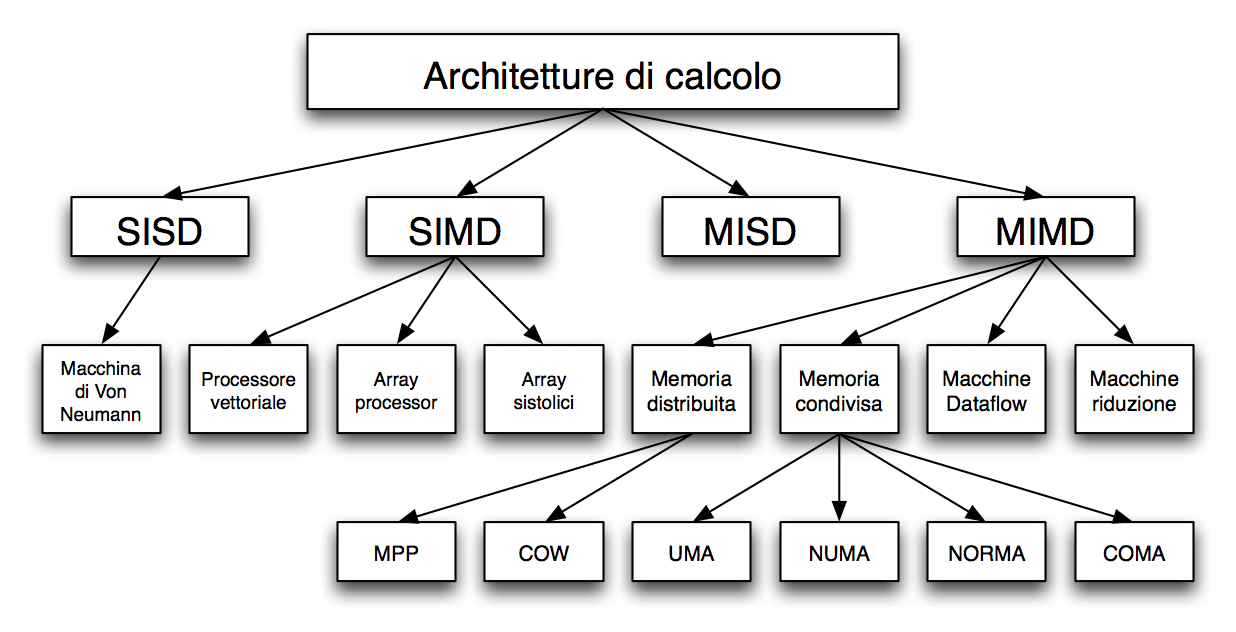
\includegraphics[width=0.5\columnwidth]{Immagini/flynn} 
\caption[Tassonomia di Flynn]{La tassonomia di Flynn}
\label{fig:flynn} 
\end{figure}

I computer attualmente in commercio sono basati sull'architettura di Von Neumann (SISD), 
cio� un architettura in cui non � presente nessun tipo di parallelismo e le
operazioni vengono eseguite sequenzialmente su un flusso di dati singolo.
Sia le architetture SIMD (Single Instruction stream Multiple Data stream) che le
architetture MIMD (Multiple instruction stream Multiple Data stream) descritte
in precedenza, si basano sulla filosofia del parallelismo.

Una sottocategoria delle architetture MIMD (Multiple Instruction stream Multiple
Data stream) � l'architettura SPMD (Single Program Multiple Data).
La sua tecnica � programmata per raggiungere il parallelismo. Si tratta di
lanciare pi� istanze dello stesso programma su diversi insiemi di dati.

Le GPU (graphics processing units), richiamate in precedenza, sono l'esempio di
architetture SIMD, mentre i processori pi� comuni sono un esempio di architettura MIMD.


%**********************************************
%												-
%		     COMUNICAZIONE   					-
%												-
%**********************************************

\section{Modelli di comunicazione}

Tra le basi del parallelismo esiste l'opportunit� di far comunicare i diversi
\textit{tasks} paralleli. Esistono due forme diverse di comunicazione:
\begin{itemize}
	\item accesso ad uno spazio di memoria condivisa
	\item scambio di messaggi
\end{itemize}

 \subsection{Memoria condivisa}
Questo tipo di architetture fanno si che tutte le unit�di calcolo presenti
accedono allo stesso spazio di memoria.
I cambiamenti eseguiti da una singola unit�di calcolo devono essere visibili
anche dalle altre unit�di calcolo.
Possiamo distinguere due diversi tipi di accesso alla memoria:

\begin{itemize}
	\item UMA (Uniform Memory Access): tutti i processori accedono allo spazio di
	memoria condivisa allo stesso tempo.
In questo caso l'hardware deve assicurare la coerenza della cache in modo tale
che tutte le unit�di calcolo possano vedere le modifiche eseguite dagli altri
processori, cos� da evitare accessi ai dati non aggiornati.
Questo meccanismo � chiamato \textbf{\textit{cache coherence}}.
(Fig.\ref{fig:uma})
	\item NUMA (Non Uniform Memory Access): tutti i processori possono accedere
alla loro memoria locale in modo estremamente rapido, tuttavia accedono pi�
lentamente alla memoria condivisa e alla memoria degli altri processori.
Anche in questo caso troviamo il meccanismo di {\textit{cache coherence}} per
garantire l'accesso coerente ai dati in memoria. (Fig. \ref{fig:numa})
\end{itemize}

Grazie alla presenza di memorie condivise, risulta molto semplice programmare
algoritmi paralleli. Tuttavia ci sono dei punti critici da gestire, come ad
esempio il meccanismo di lettura e scrittura. Per quanto riguarda il meccanismo
di lettura, pu� avvenire in modo del tutto trasparente poich� non apporta
inconsistenze nella memoria condivisa, ci� non accade per la scrittura, dove si
ha bisogno di ulteriori meccanismi per l'accesso \textbf{esclusivo}.
I paradigmi che supportano il modello di comunicazione a memoria condivisa (e.g.
POSIX threads, OpenMP) forniscono strutture per la sincronizzazione come
\textit{lock, barriere, semafori} e cos� via.


\begin{figure}[tb]
\centering
\subfloat[UMA.]
{\label{fig:uma}
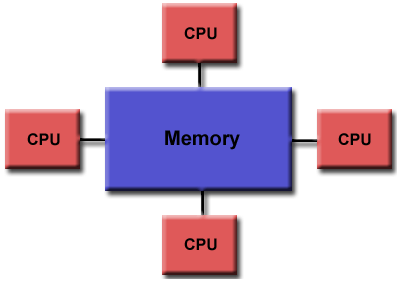
\includegraphics[width=.45\columnwidth]{Immagini/uma}} \quad
\subfloat[NUMA.]
{\label{fig:numa}
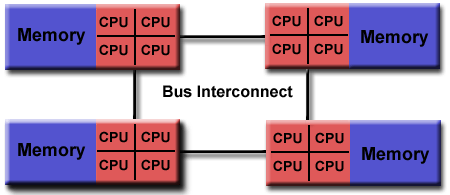
\includegraphics[width=.45\columnwidth]{Immagini/numa}} \\
\caption[UMA e NUMA]{UMA e NUMA.}
\end{figure}

 \subsection{Memoria distribuita}

Le architetture a memoria distribuita prevedono diverse unit�di calcolo, ognuno
dei quali possiede un proprio spazio di memoria.
Le unit�di calcolo possono essere composte da un singolo processore o da un
sistema multiprocessore con uno spazio di memoria condiviso.
I processi in esecuzione comunicano attraverso uno scambio di messaggi.
Grazie a questa interazione, i processi possono scambiarsi dati, assegnare task
e sincronizzare i processi.
L'architettura MIMD viene supportata da questo modello di comunicazione, ma
nella maggior parte dei casi, le implementazioni basate sullo scambio dei
messaggi sono implementati con l'approccio SPMD.

Le operazioni di base che un processo pu� eseguire sono l'invio e la ricezione
dei messaggi.
Nello scambio di messaggi � necessario anche specificare chi � il mittente e
chi il destinatario del messaggio, per questo il sistema offre un meccanismo di
assegnazione di un ID univoco ad ogni processo, in modo da distinguerlo da tutti
gli altri. Altre funzionalit� presenti in questo paradigma sono il
\textit{whoami} e il \textit{numProc}. Il primo permette ad ogni processo di
conoscere il proprio ID univoco, mentre il secondo consente ad ogni processo di
conoscere il numero di processi in esecuzione.

Oggi ci sono diversi framework che consentono lo scambio di messaggi.
Uno di questi � MPI (Message Passing Interface) che supporta tutte le operazioni
citate in precedenza.

 \subsection{Sistemi ibridi}

Le architetture basate sui sistemi ibridi non sono nient'altro che un mix delle
due architetture viste in precedenza.
Immaginiamo di avere un numero \textit{N} di processi. Solo un sottoinsieme di
processi avranno accesso alla memoria condivisa.
Per accedervi possono utilizzare ad esempio un paradigma di programmazione
parallela a memoria condivisa (e.g OpenMP).
Ogni processo che ha accesso alla memoria condivisa, pu� comunicare i dati
tramite il paradigma del Message Passing agli altri processi che non vi hanno
accesso. In questo modo entrano in gioco le due diverse architetture sfruttando
i vantaggi di entrambe.

\begin{figure}[b] 
\centering 
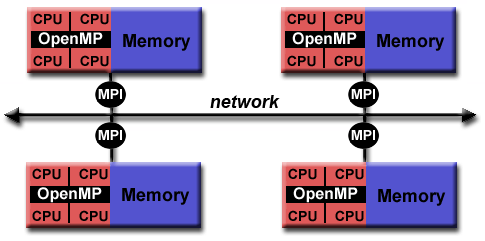
\includegraphics[width=0.5\columnwidth]{Immagini/hybrid_model} 
\caption[Sistema Ibrido]{Esempio di sistema ibrido.\\}
\label{fig:hybrid_model} 
\end{figure}


%**********************************************
%												-
%		PROGETTAZIONE DI UN ALGORITMO PARALLELO		-
%												-
%**********************************************

\section{Progettazione di un algoritmo parallelo}

Fino ad ora si � descritto in modo generico le strutture, le basi dei paradigmi
e le architetture per sistemi paralleli, ma la progettazione di un algoritmo
parallelo � la parte che interessa di pi� un programmatore.
Progettare un algoritmo parallelo implica uno studio totalmente diverso dalla
progettazione di un algoritmo sequenziale.
Come abbiamo gi� visto, entrano in gioco diverse operazioni per raggiungere
l'output desiderato.
Molte guide di calcolo parallelo evidenziano le seguenti problematiche per la
progettazione di un algoritmo parallelo \textit{nontrivial} \cite{ITPC:2003}:

\begin{itemize}
	\item Identificazione della porzione di lavoro che pu� essere eseguita
	concorrentemente.
	\item Mapping dei task su pi� processi in parallelo
	\item Assegnare i dati relativi al programma.
	\item Gestire gli accessi alla memoria condivisa
	\item Sincronizzare le unit�di calcolo durante l'esecuzione.
\end{itemize}
 
Di solito ci sono diverse scelte da fare durante la progettazione, ma spesso si
possono prendere decisioni progettuali anche basandosi sull'architettura a
disposizione o in base al paradigma di programmazione utilizzato.

\subsection{Tecniche di decomposizione}

La decomposizione � il processo di dividere la computazione in piccole parti che
potenzialmente possono essere eseguite in parallelo.
I task sono unit� di computazione nei quale la computazione principale viene
suddivisa.
Ci sono casi in cui alcuni task per poter iniziare la propria attivit� hanno
bisogno dell'output di altri task, cos� da formare una relazione di dipendenza.
Questo genere di relazione di dipendenza nel parallel computing viene
rappresentata dal \textbf{\textit{task-dependency graph}}.
Il grafo delle dipendenze � un grafo diretto e aciclico nel quale ogni nodo
rappresenta un task e gli archi rappresentano la dipendenza tra i nodi.
Quest'ultimo risulter�molto utile nei casi in cui si debbano prendere alcune
scelte di progettazione dell'algoritmo, in particolare fornir� informazioni
importanti sulla strategia da utilizzare per la suddivisione dei tasks.
Un altro importante concetto per la suddivisione dei task � la
\textbf{granularit�}. Distinguiamo due tipi di granularit�:
\begin{description}
	\item [Suddivisione a granularit� fine] quando la decomposizione produce
	un numero consistente di task ma di piccola dimensione.
	\item [Suddivisione a granularit� grossa] quando la decomposizione produce un
	basso numero di task ma di grande dimensione.
\end{description}

Il numero di task che possono essere eseguiti in parallelo invece � detto
\textbf{grado di concorrenza}.

Gli esempi pi� comuni di suddivisione dei task � rappresentato dai calcoli
eseguiti su matrici. Supponiamo di avere a disposizione 4 unit�di calcolo, e il
task principale da eseguire � una semplice somma di tutte le celle della
matrice. Possiamo decomporre la nostra matrice in 4 parti uguali (se �
possibile), e assegnarne una per ogni processo a disposizione. Ipoteticamente
l'algoritmo sar� 4 volte pi� veloce rispetto alla versione sequenziale.

\begin{figure}[tb] 
\centering 
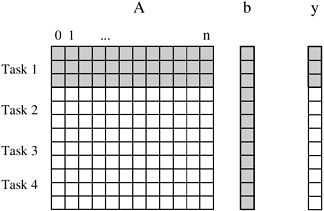
\includegraphics[width=0.5\columnwidth]{Immagini/matrix_dec} 
\caption[Decomposition example]{Suddivisione di una moltiplicazione tra una
matrice e un vettore in 4 diversi task.\\}
\label{fig:matrix_dec} 
\end{figure}

Spesso anche il fattore di interazione tra i processi � un dato da non
sottovalutare in una buona progettazione di un algoritmo parallelo. Come nel
caso della fig. \ref{fig:matrix_dec} tutti i task hanno bisogno di accedere
all'intero vettore \textit{b}, e nel caso in cui si ha una sola copia del
vettore, i task devono obbligatoriamente iniziare a comunicare tra di loro
tramite messaggi per accedere alle informazioni. Questa relazione tra i task
viene rappresentata da un altro grafo: il \textbf{\textit{task-interaction graph}}.

L'interazione tra task � un fattore che limita molto la speedup di un algoritmo
parallelo.

\begin{figure}[tb] 
\centering 
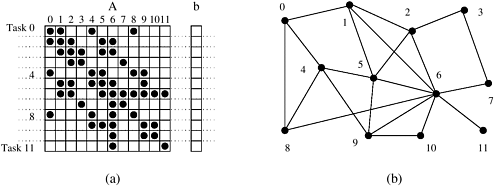
\includegraphics[width=0.5\columnwidth]{Immagini/matrix_int} 
\caption[Task-interaction graph]{Esempio di un grafo delle interazioni tra i task.\\}
\label{fig:matrix_int} 
\end{figure}

Vediamo insieme ora le cinque differenti tecniche di decomposizione.

\begin{figure}[b] 
\centering 
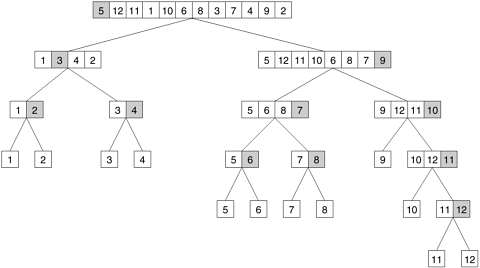
\includegraphics[width=0.5\columnwidth]{Immagini/dec_ric} 
\caption[Decomposizione ricorsiva]{Esempio di decomposizione ricorsiva: il quicksort.\\}
\label{fig:dec_ric} 
\end{figure}



\subsubsection{Decomposizione ricorsiva}
La decomposizione ricorsiva � una tecnica per applicare la concorrenze in
problemi che possono essere risolti tramite la strategia del divide-et-impera.
La prima divisione consiste nel dividere il problema principale in sottoproblemi
indipendenti. Ognuno dei sottoproblemi generati viene risolto ricorsivamente
applicando la stessa tecnica.

\begin{figure}[b] 
\centering 
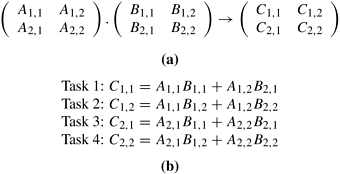
\includegraphics[width=0.5\columnwidth]{Immagini/dec_dat} 
\caption[Decomposizione dei dati]{Esempio di decomposizione dei dati.\\}
\label{fig:dec_dat} 
\end{figure}

\subsubsection{Decomposizione dei dati}
La decomposizione dei dati � una tecnica che pu� essere applicata seguendo
diversi approcci.

\begin{itemize}
	\item Partizione dell'output dei dati: si sceglie questa tecnica nel caso in
	cui gli output possono essere calcolati indipendentemente uno dall'altro,
	senza aver bisogno di rielaborare il risultato finale. Ogni problema viene
	suddiviso in task, dove ad ognuno viene assegnato il compito di calcolare
	esattamente una porzione di output. (Fig. \ref{fig:dec_dat})
	\item Partizione dell'input dei dati: si sceglie questa tecnica nel caso in
	cui il risultato atteso � un dato singolo (eg. minimo, somma tra numeri). Si
	creano task per ogni partizione dell'input, ed ognuno di loro proseguono nella
	computazione nel modo pi� indipendente possibile. E' quasi sempre necessario
	dunque ricombinare i risultati alla fine della computazione.
\end{itemize}


\subsubsection{Decomposizione esplorativa}
La decomposizione esplorativa � una tecnica utilizzata per decomporre problemi
nei quali per trovare la soluzione viene generato uno spazio di ricerca. Lo
spazio di ricerca � suddiviso in diverse parti e in ciascuna di queste in
parallelo si cerca la soluzione. Quando un processo trova la soluzione, tutti
gli altri processi si interrompono.


\subsubsection{Decomposizione speculativa e ibrida}
La decomposizione speculativa � usata quando un programma pu� prendere diverse
scelte che dipendono dall'output dello step precedente. Un esempio lampante � il
caso dell'istruzione \textit{switch} in C, prima che l'input per lo switch sia
arrivato. Mentre un task computa un ramo dello switch, gli altri task in
parallelo possono prendere a carico gli altri rami dello switch da computare.
Nel mondo in cui l'input arriva allo switch viene preso in considerazione
solamente il ramo corretto mentre gli altri possono essere scartati.

La decomposizione ibrida invece, si occupa di combinare diverse tecniche ai fini
di migliorare le performance ulteriormente. E' struttrata in pi� step, dove per
ogni step si applica una tecnica di decomposizione diversa.

\subsection{Tecniche di mapping}

Una volta decomposto il problema in task, c'� la necessit�di creare un
mapping tra i task e i processi. Il mapping � una fase molto importante e
delicata ai fini di una buona performance. L'obiettivo da raggiungere �
minimizzare in modo consistente l'overhead che si crea nell'esecuzione dei task
in parallelo. Tra le principali fonti di \textbf{overhead} troviamo
l'interazione tra i processi durante il periodo di esecuzione e il tempo in cui
diversi processi non effettuano nessuna operazione. Frequentemente, per limitare
la comunicazione tra i processi, nel caso in cui ci troviamo di fronte a task di
piccole dimensioni, si pu� scegliere di accorpare pi� task assegnandole ad un
unico processo. Questa pu� sembrare una scelta logica, a volte potrebbe anche
essere la scelta corretta ma, creare un processo pi� corposo di un altro
potrebbe scalfire il \textit{load balancing}.

Proprio per questo la scelta di un corretto mapping potrebbe contrastare questo
genere di problematiche, cos� da diventare determinante ai fini del
raggiungimento di una buona performance. Distinguiamo due tipi di tecniche di mapping:

\begin{itemize}
\item Mapping statico
\item Mapping dinamico
\end{itemize}

Descriviamo brevemente i due differenti approcci.

La tecnica di mapping statico assegna i task ai processi prima dell'inizio di
esecuzione dell'algoritmo. In genere questa tecnica � utilizzata quando
l'euristica dei task non � computazionalmente costosa, dunque gli algoritmi sono
pi� facili da progettare e implementare.

La tecnica di mapping dinamico invece distriuisce il lavoro durante l'esecuzione
del programma. Scegliamo questa tecnica quando la dimensione dei task �
sconosciuta e non si possono prevedere dunque le possibilit� per un mapping
ottimale \cite{ITPC:2003}.

\subsection{Modelli di un algoritmo parallelo}

In questo paragrafo si mostreranno i differenti modelli utilizzati per
implementare un algoritmo parallelo.

\begin{description}
\item [Dati in parallelo] E' il pi� sempice dei modelli. Questo tipo di
parallelismo � il risultato di operazioni identiche applicate concorrentemente
in diversi elementi di dati. Si pu� reallizzare questo modello sia con un
architettura a memoria condivisa sia utilizzando il paradigma del message-passing.
\item [Task graph] E' un modello basato sul concetto del task-dependency graph.
A volte il grafo delle dipendenze pu� essere banale o non banale, e le
interazioni tra i processi sono numerose. Questo modello � utilizzato per
risolvere i problemi in cui la quantit�di dati associata ai task � pi� grande
rispetto alla quantit� di calcolo ad essi associato. Un esempio basato sul
questo modello comprende il quicksort parallelo come tanti altri algoritmi
basati sul divide-et-impera.
\item [Master-Slave] E' uno dei pi� famosi modelli per progettare un algoritmo
parallelo. Con questo modello uno o pi� processi vengono identificati come
\textit{master} e hanno il compito di distribuire il lavoro agli altri processi,
definiti \textit{slave}. Questo modello pu� essere accompagnato sia da una
memoria condivisa che dal paradigma del message-passing. Spesso si usa questo
modello quando si ha bisogno di gestire le diverse fasi di un algoritmo, in
particolare per ogni fase un compito del master potrebbe comportare la
sincronizzazione di tutti gli slaves. Bisogna essere comunque parsimoniosi se si
decide di utilizzare questo modello, poich� pu� comportare facilmente colli di
bottiglia che porterebbero ad una bassa performance.
\end{description}

\begin{figure}[tb] 
\centering 
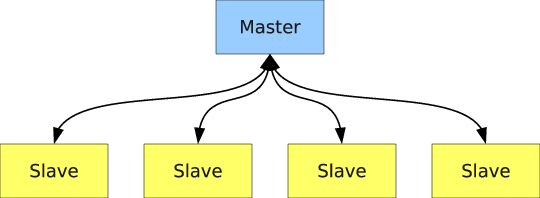
\includegraphics[width=0.5\columnwidth]{Immagini/master-slave} 
\caption[Modello Master-Slave]{Il modello Master-Slave.\\}
\label{fig:master-slave} 
\end{figure}


%**********************************************
%												-
%			MISURE DI PERFORMANCE					-
%												-
%**********************************************

\section{Misure di performance}
\label{par:misure_performance}
Fino ad ora si � parlato di perfomance, di parallelizzare un algoritmo in modo
da renderlo pi� veloce. Nel parallel computing per definire il concetto di
velocit�e di performance migliore si utilizzano diverse misure, che analizzano
e permettono di valutare gli algoritmi, le architetture utilizzate e i benefici
del parallelismo. Intendiamo misura di perfomance:
\begin{itemize}
\item Il tempo di esecuzione
\item L'overhead totale
\item Lo speedup
\item L'efficienza
\end{itemize}

Andiamo a descrivere ora, il significato di queste misure

Il \textbf{tempo di esecuzione} \textit{T} � il tempo effettivo che passa tra il
momento in cui viene lanciato l'algoritmo e il momento in cui termina. Per gli
algoritmi paralleli il tempo di esecuzione il tempo che passa tra il momento in
cui inizia la computazione parallela fino al momento in cui l'ultimo processore
termina la computazione. Questa pu� essere considerata come una prima
valutazione del parallelismo.

L'\textbf{overhead} totale nel parallel computing � il tempo di esecuzione
impiegato collettivamente da tutti i processori rispetto al tempo richiesto dal pi� veloce algoritmo sequenziale per risolvere il problema.

\begin{equation}
T_o = pT_p - T_s
\end{equation}
dove $p$ � il numero di unit� di calcolo, $T_p$ � il tempo parallelo e $T_s$ �
il tempo sequenziale.

Le due misure pi� importanti tra quelle citate sono la \textit{speedup} e l'\textit{efficienza}. 
Nel valutare un algoritmo spesso si vuole sapere qual � il guadagno, in
termini di performance, di un'implementazione parallela rispetto ad
un'implementazione seriale. Lo \emph{speedup} quantifica i benefici nel
risolvere un problema in parallelo e pu� essere definito come il rapporto tra il
tempo $T_s$ necessario per risolvere il problema su una singola unit� di
calcolo e il tempo $T_p$ per risolvere lo stesso problema su un calcolatore
parallelo con $n$ identiche unit� di calcolo. 
\begin{equation}
S = \frac{T_s}{T_p}
\end{equation}
In genere $T_s$ � il tempo di esecuzione del pi� veloce algoritmo sequenziale
conosciuto, in grado di risolvere il problema dato. In teoria, lo speedup non
supera mai il numero di unit� di calcolo $n$. Se $T_s$ rappresenta il tempo del
miglior algoritmo sequenziale, per ottenere uno speedup pari a $n$, avendo a
disposizione $n$ unit� di calcolo, nessuna di esse deve impiegare un tempo
maggiore di $\frac{T_s}{n}$. Uno speedup maggiore di $n$ � possibile solo se
tutte le unit� di calcolo hanno un tempo di esecuzione minore di
$\frac{T_s}{n}$. In questo caso una singola unit� di calcolo potrebbe emulare le
$n$ unit� di calcolo e risolvere il problema con un tempo minore di $T_s$.
Questa � una contraddizione poich� $T_s$ � il tempo di esecuzione del miglior
algoritmo sequenziale. In pratica, � per� possibile avere uno speedup maggiore
di $n$ (speedup superlineare). Generalmente questo � dovuto a caratteristiche
dell'hardware che mettono l'implementazione sequenziale in svantaggio rispetto a
quella parallela. Ad esempio, � possibile che la cache di una singola unit� di
calcolo non sia abbastanza grande da contenere tutti i dati da elaborare,
quindi, le sue scarse prestazioni sono dovute all'utilizzo di una memoria con
un accesso lento rispetto a quello della memoria cache. Nel caso
dell'implementazione parallela i dati vengono partizionati e ogni
parte � abbastanza ridotta da entrare nella memoria cache dell'unit� di calcolo
alla quale � stata assegnata. Questo spiega come in pratica sia possibile avere
uno speedup superlineare.

L'\emph{efficienza} � una misura di prestazione legata allo speedup. Come
menzionato precedentemente, la parallelizzazione di un'algoritmo introduce un
overhead dovuto alla comunicazione tra i processi e ai processi che entrano in
uno stato di idling. Per questo motivo � molto difficile raggiungere uno speedup
pari al numero di unit� di calcolo. L'efficienza quantifica la quantit� di
lavoro utile (tralasciando i tempi dovuti a overhead) effettuato dalle $n$ unit�
di calcolo ed � definita come il rapporto tra lo speedup e $n$.

\begin{equation}
E = \frac{S}{n}
\end{equation}


%**********************************************
%												-
%			LINGUAGGI DI PROGRAMMAZIONE			-
%												-
%**********************************************
\section{Linguaggi di programmazione}
Esistono diversi linguaggi di programmazione e paradigmi di programmazione che
consentono l'utilizzo del parallel computing durante l'implementazione di un
algoritmo. Tra i pi� utilizzati troviamo sicuramente OpenMP e MPI.
Nel prossimo paragrafo vedremo sommariamente come funziona OpenMP.

\subsection{OpenMP}
OpenMP � uno standard che offre funzionalit� per creare algoritmi paralleli in
uno spazio di memoria condiviso. Supporta dunque la concorrenza, la
sincronizzazione e altre funzionalit� utili per una corretta implementazione di
un algoritmo parallelo su memoria condivisa.
OpenMP per la sua semplicit� � molto usato, e qualche volta riesce a
raggiungere risultati ottimi con speedup interessanti.
Il suo utilizzo si basa sulla dichiarazione della seguente direttiva:
\begin{center}
\textbf{ \#pragma omp directive [clause list] } 
\end{center} 
Il programma si esegue sequenzialmente finch� non trova la direttiva
\textbf{\textit{parallel}}. Questa direttiva � responsabile della creazione di
un gruppo di \textit{threads} che devono eseguire in parallelo l'algoritmo.
Il prototipo della direttiva parallel � il seguente:
\begin{center}
\textbf{ \#pragma omp parallel [clause list] } 
\end{center}
La lista di clausole � utile per aggiungere gradi di libert� all'utente
nell'utilizzo della concorrenza.
Ad esempio nel caso in cui la parallelizzazione e la conseguente creazione di
pi� threads in parallelo debba avvenire solo in determinati casi, si pu�
utilizzare la clausola:
\begin{center} 
\textbf{ if ( \textit{espressione} ) }
\end{center}
In questo caso solo se l'\textit{espressione} � vera si user� la direttiva
\textit{parallel}.
Un altra clausola utilizzata � 
\begin{center} 
\textbf{num\_threads (int)}
\end{center}
Questa specifica il numero di threads che devono essere creati ed eseguiti in
parallelo.
Nel caso in cui si vogliano utilizzare delle variabili private per ogni thread
si pu� utilizzare la clausola:
\begin{center} 
\textbf{private ( lista delle variabili )}.
\end{center}
che specifica la lista delle variabili locali per ogni thread, cio� ogni thread
possiede una copia di ognuna di queste variabili specificate in questa clausola.
Le clausole che mette a disposizione OpenMP sono molteplici, tra queste troviamo
la causola \textbf{\textit{reduction(operazione: variabile)}} che come si pu�
intuire applica una particolare operazione aritmetica ad una variabile.

Tra le direttive di OpenMP la pi� interessante � la direttiva \textbf{for}. La
forma generale di questa direttiva �:
\begin{center} 
\textbf{\#pragma omp for [clause list] }. \\
 /* ciclo di for */
\end{center}
Questa � utilizzata per dividere lo spazio delle iterazioni parallele attraverso
i threads a disposizione.

In generale OpenMP offre veramente decine di funzionalit� da poter utilizzare e
l'aspetto migliore di questo paradigma � sicuramente la semplicit� della sua
implementazione e l'integrazione con l'algoritmo parallelo. In ultimo, ecco un
semplice esempio di parallelizzazione tramite OpenMP di un algoritmo sequenziale:

\medskip
\lstinputlisting[caption={Esempio di utilizzo di OpenMP.},
label=lst:openmp, style=input]{code/openmp.c}

%\subsection{MPI}

%**********************************************
%												-
%				GPGPU PROGRAMMING				-
%												-
%**********************************************

\section{Nuovi approcci al calcolo parallelo: GPGPU computing}

La GPU (Graphics Processing Unit) � un processore grafico specializzato nel
rendering di immagini grafiche. Viene utilizzata generalmente come coprocessore
della CPU, infatti � tipicamente una componente della CPU in un circuito
integrato, ma da alcuni anni la sua potenza di calcolo ha suscitato parecchio
interesse nel campo scientifico. Le numerose ricerche hanno portato
all'implementazione come circuito indipendente dotato di pi� \textit{cores}.
Sebbene le GPU operino a frequenze pi� basse rispetto alle CPU sin dai primi
anni del nuovo millennio esse superano le CPU nel calcolo di operazioni in
floating point (FLOPS) e, ad oggi la velocit� di calcolo delle GPU � quasi
dieci volte superiore quelle delle CPU.
Prima del 2006, le GPU difficilmente venivano usate per scopi diversi dal
rendering grafico poich� per accedere a questi dispositivi i programmatori
avevano a disposizione soltanto API per la grafica (ad esempio OpenGL
\cite{OpenGL:2004}). GPGPU (general purpose computing on graphic processing
unit) � il termine che viene usato per indicare l'utilizzo delle GPU in ambiti
diversi dal rendering grafico. Questa tecnica si diffuse nel 2007 grazie al
rilascio di CUDA \cite{CUDA:2007} da parte NVIDIA, che permetteva ai
programmatori di sviluppare applicazioni parallele senza utilizzare le API
grafiche. Oltre a questo NVIDIA inizi� ad inserire nei propri dispositivi delle
componenti hardware apposite a supporto della programmazione parallela.

\begin{figure}[H] 
\centering 
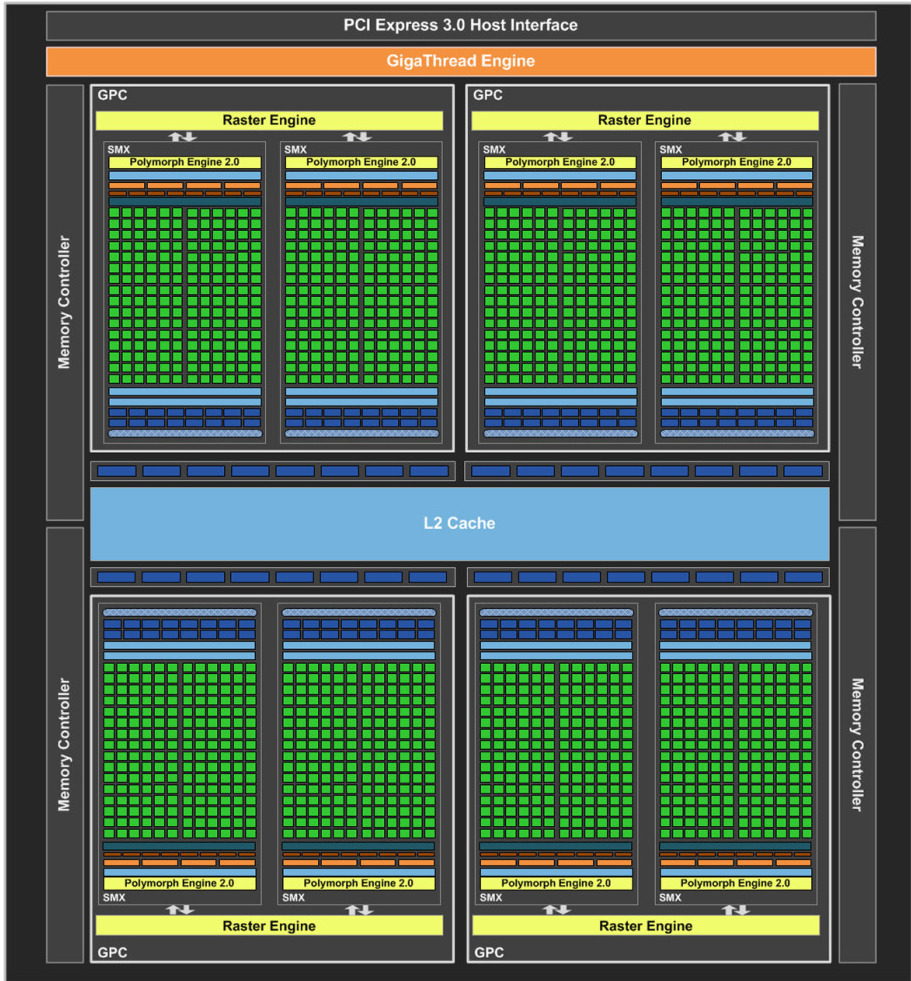
\includegraphics[width=0.5\columnwidth]{Immagini/arch_kepler} 
\caption[Architettura Kepler]{Architettura Kepler (GTX 680).\\}
\label{fig:arch_kepler} 
\end{figure}

La figura \ref{fig:arch_kepler} rappresenta l'architettura di una tipica GPU
CUDA. La struttura � composta da un insieme di \emph{streaming multiprocessor}
(SM) divisi in blocchi (Nella figura \ref{fig:arch_kepler} ci sono due SM
per ogni blocco). Ogni SM � composto da un insieme di \emph{streaming
processors} che condividono la memoria cache. Ogni GPU ha a disposizione alcuni
gigabytes di Graphic Double Data Rate DRAM, anche detta memoria globale. Questo
tipo di memoria � diversa dalla normale memoria DRAM poich� � progettata per
contenere dati relativi alla grafica. Nel caso di applicazioni grafiche contiene
informazioni relative ad immagini e texture usate per il rendering 3D. In ambito
GPGPU viene sfruttata per la sua ampia larghezza di banda al costo
di una maggiore latenza rispetto alla normale memoria DRAM. Con l'aumentare
della disponibilit� di memoria delle GPU prodotte, le applicazioni tendono a
memorizzare i dati nella memoria globale minimizzando le interazioni con la
memoria del sistema. Le GPU sono particolarmente adatte a risolvere problemi che
possono essere modellati con un approccio SIMD (vedi paragrafo
\ref{par:flynn}) e che contengono una gran quantit� di calcoli
aritmetici \cite{Kartashev}. Generalmente lo stesso programma viene eseguito per
ogni dato da elaborare e la latenza dovuta agli accessi alla memoria globale
viene ``nascosta'' dalla grande quantit� di calcoli.
% !TEX encoding = UTF-8
% !TEX TS-program = pdflatex
% !TEX root = ../Tesi.tex
% !TEX spellcheck = it-IT

%************************************************
\chapter{CUDA - Compute Unified Device Architecture}
\label{cap:CUDA}
%************************************************

\section{Introduzione}
Quasi nove anni fa, nel Novembre 2006  la \textbf{NVIDIA Corporation} ha
rilasciato CUDA, una piattaforma (hardware e software insieme) che permettono di
utilizzare linguaggi di programmazione ad alto livello (Ad es. \textbf{C},
\textbf{C++}, \textbf{Java}) per implementare codice parallelo per risolvere
problemi molto complessi a livello computazionale in una maniera efficiente
rispetto alle normali CPU.

\begin{figure}[h] 
\centering 
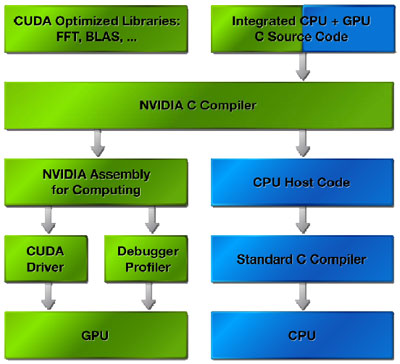
\includegraphics[width=0.5\columnwidth]{Immagini/cuda_compiler} 
\caption[Compilatore NVCC]{Struttura di Nvidia C Compiler.\\}
\label{fig:cuda_compiler} 
\end{figure}

CUDA � molto utilizzato poich� � un sistema completo e anche molto semplice da
capire ed utilizzare. Sopratutto quest'ultimo particolare � di importante
rilevanza, dato che attualmente le alternative a CUDA, come OpenCL, risultano
essere molto pi� complesse a livello implementativo e di leggibilit� del
codice.
Come illustrato in figura \ref{fig:cuda_compiler}, NVIDIA fornisce un
compilatore capace di riconoscere le istruzioni CUDAma l'implementazione di un
programma parallelo avviene utilizzando codice sorgente sia per CPU che per GPU.
Il compilatore NVIDIA C (\textit{nvcc}) dunque, identifica il tipo di istruzione
richiamando i compilatori di riferimento gestendo cos� questa convivenza.
  
\section{Architettura hardware}

Oggi sul mercato delle schede video possiamo trovare innumerevoli tipi di
device, e i computer moderni referibilmente posseggono una scheda video
dedicata. In particolare la \textbf{Nvidia Corporation} ha creato anche diverse
architetture hardware per soddisfare ogni tipo di richiesta. Quelle conosciute
sono le architetture \textbf{Kepler}, \textbf{Fermi} e \textbf{Tesla}.
L'architettura Kepler � quella pi� utilizzata nei computer in commercio con
scheda grafica NVIDIA.

 In generale, le architetture GPU NVIDIA, sono composte da un array di
 \textit{Streaming Multiprocessors (SMs)}. Lo Streaming Multiprocessors �
 progettato per eseguire centinaia di threads in parallelo e contiene un
 determinato numero di Streaming Processors (SP). Gli Streaming processors sono
 anche chiamati \textit{CUDA cores} e il loro numero dipende dalla capacit� del
 device installato.
 
 \subsection{Compute capability}
Ogni device possiede un \textit{revision number} che possiamo definire come la
\textbf{compute capability} del device, e determina l'insieme di funzionalit�
che possono essere usate nell'implementazione di codice parallelo in CUDA.
La compute capability � definita dal pi� alto numero di revision number e il
minor numero di revision number. Nel caso in cui devices diversi abbiano il pi�
alto revision number posseggono la stessa architettura. Il pi� alto numero di
revision number per le architetture Kepler � 3, per i devices basati su
un'architettura Fermi � 2, mentre per i device con architettura Tesla 1. Il
numero minore di revision number invece, corrisponde al miglioramento del core
dell'architettura che spesso porta a nuove funzionalit� da poter utilizzare
tramite le API fornite appunto da NVIDIA.

\subsection{Architettura Kepler}
L'architettura Kepler � stata progettata e successivamente lanciata nel 2010
insieme all'architettura Fermi. La prima GPU basata sull'architettura Kepler si
chiamava ``GK104" in cui ogni unit� interna � stata progettata ai fini di
avere la miglior performance per watt (perf/watt). Alcuni esperti hanno
affermato che la GK104 Kepler � la GPU pi� potente per la computazione e il
rendering grafico dei videogames.

Inizialmente la GPU utilizzata per questo lavoro di tesi � stata la NVIDIA
GeForce GT 750M basata anch'essa su un architettura Kepler. Il core in
particolare � il ``GK107" che offre due shader di blocchi, chiamati
\textbf{SMX}, ognuno dei quali ha 192 shaders per un totale di 384 shader cores
con una velocit� di 967 MHz.

\begin{figure}[h] 
\centering 
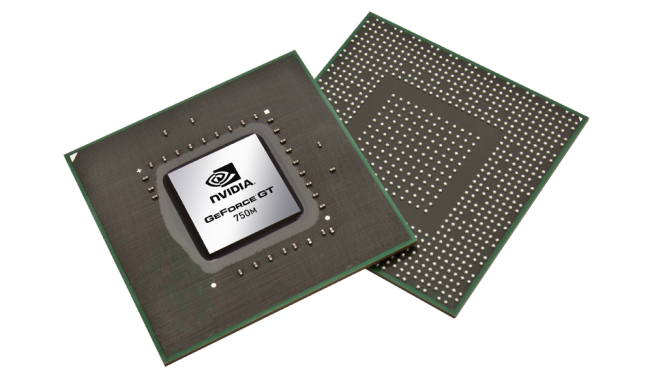
\includegraphics[width=0.5\columnwidth]{Immagini/gt750m} 
\caption[GT 750M]{La scheda video NVIDIA GT 750-M.\\}
\label{fig:gt750m} 
\end{figure} 

\section{Interfaccia di programmazione}
Un programma CUDA consiste in una o pi� fasi che sono eseguite sia lato host
(\textbf{CPU}) che lato device (\textbf{GPU}). Le fasi in cui l'ammontare
computazionale non � eccessivo, e dunque non siamo in presenza di
parallelismo dei dati, vengono implementate lato host, mentre le fasi che
richiedono un grosso ammontare di parallelismo dei dati sono implementate lato
device. CUDA consente di creare un unico file sorgente con codice host e device
insieme. Il compilatore NVIDIA C (\textbf{nvcc} fig. \ref{fig:cuda_compiler})
separa le due diverse implementazioni durante il processo di compilazione.

Il linguaggio per scrivere codice sorgente lato device � ANSI C, esteso con
particolari \textit{keywords} per far comprendere al compilatore quali sono le
funzioni con la presenza di parallelismo. Queste funzioni sono chiamate
\textbf{\textit{kernels}}. Per utilizzare nvcc naturalmente dobbiamo essere in
possesso di una GPU NVidia correttamente montata sulla propria macchina, ma se
cos� non fosse si pu� emulare su CPU le features di CUDA per poter eseguire i
kernels (MCUDA tool etc.).

Le funzioni kernel generano un determinato di threads eseguiti in parallelo per
raggiungere il data parallelism. Ad esempio per la somma di due matrici pu�
essere implementata come un kernel dove ogni threads computa un elemento
dell'output. Il massimo del parallelismo si ha quando ad ogni threads �
associata una cella della matrice. Se la dimensione della matrice � 1000 x 1000
servono 1 milione di threads per raggiungere il nostro scopo. Lato CPU per
generare e eseguire lo scheduling di un enorme numero di threads �
particolarmente oneroso, mentre in CUDA c'� un ottimo supporto hardware da
questo punto di vista, dunque il programmatore pu� sorvolare su questo tipo di
problema.

\begin{figure}[h] 
\centering 
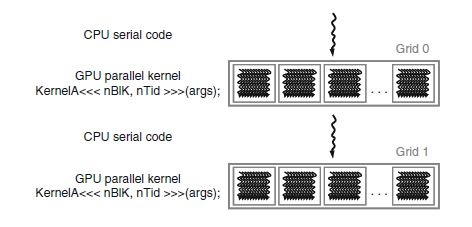
\includegraphics[width=0.5\columnwidth]{Immagini/cuda_program} 
\caption[GT 750M]{Esecuzione di un programma CUDA.\\}
\label{fig:cuda_program} 
\end{figure} 

Una tipica esecuzione di un programma CUDA � mostrata nella Fig.
\ref{fig:cuda_program}.
L'esecuzione viene eseguita a strati, la prima ad essere eseguita � la parte
host (CPU) per poi susseguirsi un insieme di strati che possono comportare anche
il lancio dei kernels nel caso ci siano parti parallelizzate. I threads sono
inglobati all'interno di \textbf{blocchi} che a loro volta sono parte di una
griglia di blocchi chiamata \textbf{grid}. Quando un kernel termina, il
programma continua con l'esecuzione lato host fino a che un nuovo kernel viene
lanciato.

\subsection{I kernel}

Come detto in precedenza, la funzione \textit{kernel} specifica il codice che
deve essere eseguito da tutti i threads lanciati nella fase parallela di un
programma CUDA. Tutti i threads lanciati in parallelo eseguono lo stesso
codice, infatti un programma CUDA non � nient'altro che l'applicazione pratica
del modello Single-Program Multiple-Data (Tassonomia di Flynn \ref{par:flynn}).
Questa tecnica � molto utilizzata nei sistemi paralleli. 

Per poter dichiarare un kernel c'� una specifica keyword di CUDA da utilizzare:
``\textbf{\_\_global\_\_}''. Questa keyword indica che la funzione � un kernel e
questa funzione richiamata dall'host generer� una griglia di threads sul device,
in particolare pu� solamente essere richiamata lato host (a
meno che non ci sia un ambiente addatto per potere utilizzare il parallelismo dinamico
\ref{par:Parallelismo_dinamico}).
CUDA genera threads suddivisi in blocchi, ed ogni blocco appartiene ad una
griglia. Lo schema � mostrato in figura \ref{fig:grid_block}.

\begin{figure}[h] 
\centering 
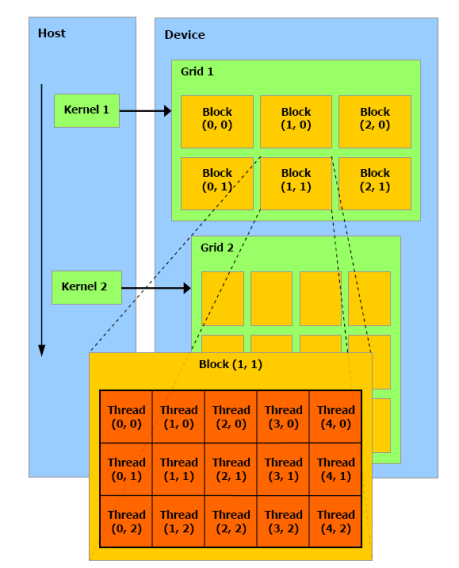
\includegraphics[width=0.5\columnwidth]{Immagini/grid_block} 
\caption[Griglie e blocchi cuda]{Esempio generico di griglie e blocchi in un
programma CUDA.\\}
\label{fig:grid_block}
\end{figure} 

In realt�, la dimensione della griglia e dei blocchi la decide il programmatore,
che organizza le diverse dimensioni in base al problema e al suo effettivo
utilizzo. Si pu� avere fino a tre dimensioni diverse (x,y,z) sia per
la griglia che per i blocchi. 
Ad ogni blocco, come per ogni threads, � assegnato un indice che pu� essere
ottenuto tramite altre keywords.   
Le keywords \textsf{threadIdx.x} e \textsf{threadIdx.y} (e in caso anche
\textsf{threadIdx.z}) si riferiscono all'indice dei threads all'interno di un
blocco. Tutti i threads eseguono lo stesso codice presente all'interno di un
kernel, quindi abbiamo bisogno di un meccanismo per distinguerli in modo da
potergli dare direttive diverse o gestire il loro comportamento.
Come per i threads anche i blocchi hanno delle specifiche keywords per risalire
alle loro coordinate. \textsf{blockIdx.x} e \textsf{blockIdx.y} hanno il compito
di ritornare il valore delle coordinate per ogni blocco. Ogni blocco deve avere
lo stesso numero di threads.

Spesso i programmatori CUDA utilizzano la \textsf{struct} \textsf{dim3} per
dichiarare la dimensione di griglie e blocchi. E' una struttura che contiene tre
diversi interi (le tre dimensioni). Ad esempio se dichiarassimo
\textsf{dim3 dimGrid(3,2,2)} vogliamo far intendere al compilatore che la
dimensione della griglia sar� tridimensionale, dove in particolare la
\textsf{x} avr� valore 3, la \textsf{y} 2 e la \textsf{z} 2. Nel caso in cui
invece dichiarassimo \textsf{dim3 dimGrid(3)} il compilatore comprende che
vogliamo solamente utilizzare una dimensione e imposter� la \textsf{y} e la
\textsf{z} ad 1 automaticamente.

Non dimentichiamo per� che le dimensioni di griglie e blocchi vengono definite
lato host e non all'interno dei kernels.

\begin{figure}[tb] 
\centering 
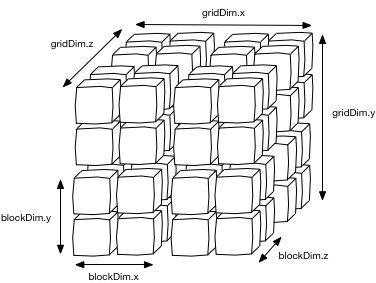
\includegraphics[width=0.5\columnwidth]{Immagini/cuda_grid} 
\caption[Griglie e blocchi cuda]{Un esempio di configurazione di griglie e
blocchi tridimensionale in CUDA.\\}
\label{fig:cuda_grid}
\end{figure} 

In ultimo � bene fare la distinzione tra i tre tipi di funzione che possono
essere dichiarate in un programma CUDA. Il primo tipo sono i kernel accompagnati
dalla keyword \textsf{``\_\_global\_\_''}, descritti in questo paragrafo, gli
altri due tipi sono \textsf{``\_\_device\_\_''} e \textsf{``\_\_host\_\_''}.
Come si pu� intuire una funzione di tipo \textsf{``\_\_device\_\_''} pu� essere
richiamata dai kernels e dunque verr� lanciata lato device, mentre
\textsf{``\_\_host\_\_''} sar� una funzione che verr� richiamata lato host, in
cui non avviene nessun parallelismo.
Nel caso in cui una funzione viene accompagnata da \textsf{``\_\_host\_\_''} e
\textsf{``\_\_device\_\_''} insieme, il compilatore genera due versioni della
funzione diverse: una per il device e un'altra per l'host.
Se una funzione invece non possiede nessuna keyword, implicitamente verr�
compilata come una funzione host.

Per lanciare un kernel, bisogna aggiungere alla chiamata a funzione la sua
configurazione definita all'interno di $ \langle\langle\langle $ e
$ \rangle\rangle\rangle $.
Al loro interno vanno definiti i parametri relativi alla dimensione di griglie
e blocchi. Un esempio lo troviamo in \ref{lst:esempio_kernel}.

Naturalmente la dimensioni di griglie e blocchi sono limitate in base alla
scheda grafica presente sulla macchina. Ad esempio sulla scheda GTX 680 il
massimo numero di threads per blocchi � 1024 e la dimensione massima di un
blocco �  \begin{math}1024 \times 1024 \times 64\end{math}.

\medskip
\lstinputlisting[caption={Esempio del lancio di un kernel con griglie e
blocchi definiti con la struct dim3.}, label=lst:esempio_kernel,
style=input]{code/esempio_kernel.c}

\subsection{La memoria}

In CUDA, host e device hanno spazi di memoria separati. L'hardware dei devices
sono dotati di random memory access propri (DRAM). Quindi per eseguire un kernel
sul device, il programmatore ha bisogno di allocare la memoria sul device e
trasferire le informazioni pertinenti ai dati sui cui si vuole agire
parallelamente dalla memoria sull'host verso la memoria allocata sul device.
\subsubsection{La shared memory}
\subsubsection{La costant memory}
\subsection{Atomicit�}
\subsection{Parallelismo dinamico}
\label{par:Parallelismo_dinamico}

\section{Tools di sviluppo}
\subsection{Nsight}
\subsection{Visual Profiler}
% !TEX encoding = UTF-8
% !TEX TS-program = pdflatex
% !TEX root = ../Tesi.tex
% !TEX spellcheck = it-IT

%************************************************
\chapter{Automi Cellulari}
\label{cap:Automi Cellulari}
%************************************************


% !TEX encoding = UTF-8
% !TEX TS-program = pdflatex
% !TEX root = ../Tesi.tex
% !TEX spellcheck = it-IT

%************************************************
\chapter{OpenCAL}
\label{cap:OpenCAL}
%************************************************

\section{Liberia per Automi Cellulari}
La modellistica � molto utilizzata negli ambienti di ricerca in diversi settori, dalla Biologia alla Geologia, dall'Ingegneria alla Bioinformatica.
Per questo motivo, negli anni, sono state sviluppate diverse metodologie per la
realizzazione di sistemi automatici e di supporto alle decisioni per la creazione di modelli e della loro
simulazione: un esempio � CAMELot \cite{CAMELOT:1996}, un ambiente di sviluppo basato su Automi Cellulari per la simulazione di processi fisici. Al contrario di CAMELot, OpenCAL (Open Cellular Automata Library) � una libreria Open Source, capace di
definire modelli di simulazione basati su Automi Cellulari complessi (CCA).

Alla base della nascita di OpenCAL troviamo la necessit� di possedere una
libreria open source, facilmente utilizzabile, che permetta all'utente di
dare completa attenzione alla definizione dell'automa cellulare trascurando il
pi� possibile i dettagli implementativi. Le funzioni, le strutture e i tipi di
dato all'interno della libreria permettono di definire un modello di Automi
Cellulari con uno spazio cellulare bidimensionale. OpenCAL supporta anche la
definizione di modelli con uno spazio cellulare tridimensionale. Tuttavia le
funzioni, le strutture e i tipi di dato usati per la definizione di un modello
2D hanno il loro corrispettivo nella versione 3D della libreria.


\section{Utilizzare OpenCAL}
Un vantaggio dell'utilizzo di OpenCAL si trova proprio sulla sua facilit� di
comprensione e di utilizzo, infatti in pochi passi � possibile definire un
modello. La gestione del modello e della simulazione sono compito delle due
\texttt{struct} principali: \texttt{CALModel2D} e \texttt{CALRun2D}. La libreria
fornisce anche funzionalit� per le operazioni di Input, Output e Buffer per la
gestione dei file (ad esempio i dati sulla morfologia).
Nelle prossime due sezioni si specificheranno la definizione di un modello e di
una simulazione nei dettagli.

\subsection{Definizione di un modello}
In una prima fase di implementazione, il programmatore deve prendersi cura della
definizione del modello. Come detto in precedenza, arrivati a questa fase
l'utente ha gi� ben chiara la progettazione dell'automa cellulare e della sua
evoluzione. Si tratta dunque di scrivere in codice le regole gi� progettate.
Grazie ad OpenCAL questo pu� essere svolto in pochi e brevi passi. E' molto
facile capire quanto possa essere oneroso impiegare del tempo per implementare
tutte le strutture necessarie ai fini di completare un programma in C/C++ adatto
per Automi Cellulari. Curarsi solamente della progettazione del
modello, lasciando ad OpenCAL il compito di gestire il \textit{core} del
problema, � senza dubbio il punto di forza della libreria.

Come anticipato in precedenza la libreria offre una struct
( \texttt{CALModel2D} ) per contenere le informazioni del modello. La funzione
\texttt{calCADef2D} permette di ottenere un'istanza di \texttt{CALModel2D}
definendone le caratteristiche. La funzione prende in input quattro diversi tipi
di parametri:
\begin{itemize}
  \item le dimensioni dello spazio cellulare
  \item la relazione di vicinanza delle celle (vicinato)
  \item la condizione ai bordi dello spazio cellulare
  \item la possibilit� di utilizzare un tipo di ottimizzazione
\end{itemize}
Le dimensioni dello spazio cellulare sono semplicemente le righe e le colonne
della matrice. La relazione di vicinanza delle celle � definita da un
enumerativo \texttt{CALNeighborhood2D} tramite cui � possibile scegliere tra i
vicinati pi� noti come Von Neumann, Moore ed il vicinato esagonale, questo non preclude la
possibilit� all'utente di definire una relazione di vicinato \textit{custom}
grazie alla funzione \texttt{calAddNeighbor2D} che riceve in input le coordinate
relative del vicino che si vuole aggiungere rispetto ad una cella centrale.


\medskip
\lstinputlisting[caption={Esempio della definizione di un modello con
vicinato di Von Neumann.}, label=lst:definitionModel,
style=input]{code/defmod.c}

In questo esempio (vedi \ref{lst:definitionModel}), possiamo osservare la
definizione di un modello con vicinato di Von Neumann, che utilizza uno spazio
di celle toroidale e non utilizza nessuna tecnica di ottimizzazione.

\medskip
\lstinputlisting[caption={Esempio della definizione di un modello con
vicinato custom definito dall'utente tramite la funzione calAddNeighbor2D.},
label=lst:definitionModel2, style=input]{code/defmod2.c}

L'ultima immagine invece mostra la definizione di un modello con un vicinato
customizzato, utilizzando la funzione \texttt{calAddNeighbor2D}.

Le condizioni ai bordi sono definite da un altro enumerativo\\
\texttt{CALSpaceBoundaryCondition}. Le due condizioni che possono essere scelte
sono: \texttt{CAL\_SPACE\_TOROIDAL} e \texttt{CAL\_SPACE\_FLAT}. Il primo
permette di scegliere uno spazio toroidale il secondo invece uno spazio non toroidale.

L'ultima condizione riguarda la possilit� di utilizzare un'ottimizzazione ai
fini di migliorare le performance del programma. Si pu� scegliere se utilizzare
le ``celle attive'' con l'opzione \texttt{CAL\_OPT\_ACTIVE\_CELLS} o meno.

Come abbiamo visto nel capitolo \ref{cap:Automi Cellulari} un modello � composto
anche da stati. In particolare nel caso degli Automi Cellulari
complessi (CCA) gli stati delle celle possono essere suddivisi in sottostati.
Dunque, OpenCAL prevede tre tipi di sottostati:
\begin{description}
  \item [\texttt{CALSubstate2Dr}] sottostati di tipo reale (\textbf{floating
  point} in C)
  \item [\texttt{CALSubstate2Di}] sottostati di tipo intero (\textbf{int} in C)
  \item [\texttt{CALSubstate2Db}] sottostati di tipo byte (\textbf{char}  in C)
\end{description}

Ogni sottostato ha due matrici linearizzate: matrice \textit{current} e matrice
\textit{next}. La prima matrice � utilizzata per leggere i valori correnti dei
sottostati mentre la seconda viene utilizzata per memorizzare i nuovi valori
calcolati. Dopo ogni step della simulazione il contenuto della matrice
\textit{next} viene copiato sulla matrice \textit{current} in modo da ottenere
il parallelismo implicito cosicch� i cambiamenti effettuati sui sottostati
non modifichino lo stato corrente delle celle finch� non si va al passo
di calcolo successivo.

Per allocare nuovi sottostati si utilizza la funzione\\
\texttt{calAddSubstate2D(b|i|r)} che restituisce un puntatore al sottostato
appena creato. Ci sono casi in cui un sottostato non deve obbligatoriamente
avere la doppia matrice, per questo c'� anche la possibilit� di allocare
sottostati con un singolo layer (dunque con la sola matrice \textit{current})
con la funzione \texttt{calAddSingleLayerSubstate2D(b|i|r)}.

\medskip
\lstinputlisting[caption={Esempio di creazione e inizializzazione di un
sottostato.}, label=lst:addsubstate, style=input]{code/addsubstate.c}

In realta quest'esempio mostra solo una parte di funzionalit� che in questa fase
si possono utilizzare. Ad esempio la libreria offre una serie di funzioni per
facilitare l'accesso ai sottostati e inizializzare le celle a valori stabiliti.

\subsection{Definizione del ciclo di esecuzione}

Il ciclo di esecuzione comprende tutto il processo di definizione e successivo
avvio della simulazione. Tramite la libreria OpenCAL � possibile infatti
aggiungere al ciclo di esecuzione le seguenti funzioni:
\begin{itemize}
  \item una funzione di inizializzazione che verr� richiamata all'inizio del
  ciclo di esecuzione.
  \item una funzione di steering che verr� richiamata alla fine di ogni passo di
  calcolo.
  \item una funzione che definisce la condizione di stop e pu� interrompere il
  ciclo di esecuzione.
\end{itemize}
Per creare un istanza della simulazione dobbiamo utilizzare la struct
\texttt{CALRun2D}. Questa struct oltre a contenere tutte le informazioni
relative alla simulazione, racchiude le funzioni citate in precedenza per
avviare un ciclo di esecuzione. 

Cos� come per il modello, la libreria mette a disposizione una funzione per la
definizione della simulazione: \texttt{calRunDef2D}.
Questa funzione prende in input il numero dei passi di calcolo da effettuare e
la modalit� di aggiornamento dei sottostati.
Dal punto di vista del numero dei passi sostanzialmente troviamo due valori da
dare in input alla funzione: il passo iniziale e il passo finale. Se il passo
finale viene impostato al valore predefinito \texttt{CAL\_RUN\_LOOP} la
simulazione non avr� mai termine. In questo caso in particolare, di solito �
definita dall'utente la condizione di stop (ad esempio quando un cratere non
emette pi� lava etc.). Per quanto riguarda l'aggiornamento degli stati questa
pu� avvenire in due modi diversi: implicita \texttt{CAL\_UPDATE\_IMPLICIT} o
esplicita \texttt{CAL\_UPDATE\_EXPLICIT}. 
Nel primo caso l'aggiornamento dei sottostati viene gestito dal ciclo di
esecuzione di OpenCAL.


\medskip
\lstinputlisting[caption={Esempio di definizione di una simulazione.},
label=lst:calrun, style=input]{code/calrun.c}

Quando che viene eseguita un processo elementare o una funzione di
supporto (init, steering, etc\ldots) appartenente al ciclo di esecuzione, il
contenuto delle matrici \textit{next} dei sottostati viene copiato nelle
matrici \textit{current}. Nel secondo caso viene gestita direttamente
dall'utente la gestione dell'aggiornamento dei sottostati. L'utente ha la possibilit� di
definire il proprio ciclo di esecuzione e la modalit� di aggiornamento dei
sottostati. Questo � reso possibile dalla funzione
\texttt{calRunAddGlobalTransitionFunc2D} che riceve in input un puntatore alla
funzione che definisce il ciclo di esecuzione dell'utente. Per aggiornare i
sottostati possiamo utilizzare due diverse funzioni: se si vogliono aggiornare
tutti i sottostati utilizziamo \texttt{calUpdate2D} se invece si vuole
aggiornare solo un numero ristretto di sottostati (o uno solo) si utilizza
\texttt{calUpdateSubstate2D(b|i|r)}. La funzione \texttt{calRun2D} permette
di eseguire una simulazione, e infine la funzione \texttt{calRunCAStep2D}
esegue un singolo passo di calcolo della simulazione per volta.

\medskip
\lstinputlisting[caption={La gestione del ciclo di esecuzione di OpenCAL.},
label=lst:ciclodiesecuzione, style=input]{code/cicloDiEsecuzione.c}

\section{Game of Life in OpenCAL}
\label{par:gol}
Il Game of Life � un automa cellulare ideato dal matematico inglese Conway nel
1970. Conway con la progettazione di questo automa cellulare voleva simulare le
dinamiche base della vita e capirne la loro evoluzione nel tempo. Il gioco della
vita in particolare � un automa cellulare ripetitivo, cio� dopo cinque step
ritorna alla sua configurazione iniziale per poi riprendere la sua evoluzione.
Lo spazio di celle del Game of Life � bidimensionale con il vicinato definito da
Moore. Una cella pu� assumere due diversi stati: viva o morta \cite{LIFE:1970}
La funzione di transizione � costituita dalle seguenti semplici regole:
\begin{enumerate}
  \item Una cella viva, rimane viva se ha esattamente due o tre celle vive nel
  suo vicinato.
  \item Una cella viva, muore per isolamento se ha meno di due celle vive nel
  suo vicinato.
  \item Una cella viva, muore per sovraffollamento se ha pi� di tre celle vive
  nel suo vicinato.
  \item Una cella morta, torna in vita se ha esattamente tre celle vive nel suo
  vicinato.
\end{enumerate}

Nella figura \ref{fig:glider} si mostra l'evoluzione del gioco della vita di
Conway con la famosa configurazione dell'aliante (\textit{glider}).

\begin{figure}[h] 
\centering 
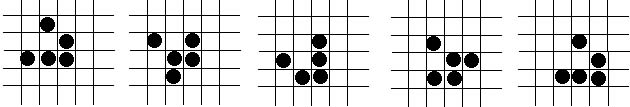
\includegraphics[width=0.7\columnwidth]{Immagini/glider} 
\caption[Gioco della vita (Glider)]{L'evoluzione del gioco della vita con
la configurazione Glider}
\label{fig:glider} 
\end{figure}

In seguito verr� mostrato l'esempio in C dell'implementazione del
\textit{Game of Life} con la libreria OpenCAL.

\medskip
\lstinputlisting[caption={Il Game of Life in OpenCAL.},
label=lst:life2D, style=input]{code/life2D.c}

Nell'esempio \ref{lst:life2D}, in circa 50 righe di codice, si implementa sia
il modello che la simulazione del Game of Life. L'estrema semplicit�
dell'implementazione mette in risalto dunque il punto di forza di OpenCAL.
La libreria permette all'utente di concentrarsi sulla definizione dell'Automa
Cellulare gestendo completamente tutti i dettagli implementativi.
L'implementazione � divisa sostanzialmente in due fasi ed in particolare nella
prima fase viene definito il modello. Usando la funzione
\texttt{calCADef2D}, si crea un'istanza di \texttt{CALModel2D} con spazio
cellulare bidimensionale toroidale e vicinato di Moore. Al modello viene
aggiunto anche un sottostato, rappresentante l'insieme degli stati delle
celle e la funzione di transizione definita dalle regole
precedentemente elencate. La seconda fase comprende la definizione del ciclo di
esecuzione. Al ciclo di esecuzione viene aggiunta una funzione di
inizializzazione che definisce la configurazione iniziale di tutte le celle.
Richiamando la funzione \texttt{calRun2D} si avvia la simulazione
e i risultati della sua esecuzione vengono infine salvati su un file dalla
funzione \texttt{calSaveSubsate2Di}.

\section{SCIARA-fv2 in OpenCAL}
\label{par:SCIARA}
Il modello computazionale pi� conosciuto, e quasi certamente il
pi� semplice a livello computazionale, � Game of life (\ref{par:gol}). La sua
implementazione � stata utile per i primi test e per i numerosi check di
correttezza della libreria. Uno degli obiettivi di questo lavoro di tesi � stato
tuttavia l'implementazione di modelli computazionalmente pi� complessi in modo
da verificare la validit� di OpenCAL e successivamente di
OpenCAL-CUDA. Il modello proposto e implementato � \textbf{SCIARA}.

La descrizione formale di SCIARA si trova al paragrafo \ref{par:sciarafv2}, in
questa sezione si mostrer� l'implementazione tramite la libreria OpenCAL.

% 
% SCIARA � un modello computazionale basato su Automi Cellulari Complessi (CCA,
% \ref{par:CCA}) che simula il fenomeno naturale di una colata lavica. Gi� da
% qualche anno � utilizzato per numerose simulazioni di casi realmente
% accaduti, tra i pi� famosi l'eruzione del Monte Etna nell'area di Nicolosi del
% 2001 \cite{SCIARA:2004} e nell'area di Valle del Bove nel 1991
% \cite{SCIARA:2001}. 
% Possiamo formalizzare l'automa cellulare complesso che definisce SCIARA nel
% seguente modo:
% 
% \begin{equation*}
% SCIARA = <Z^d, S, X, G, P, \tau, \gamma> 
% \end{equation*}
% 
% \begin{itemize}
%   \item $Z^d$ � uno spazio bi-dimensionale;
%   \item $S = S_z \times S_h \times S_t \times S^8_f$ � l'insieme finito degli
%   stati che pu� assumere una cella ottenuto dal prodotto cartesiano dei
%   sottostati. Il loro significato � rispettivamente: quota (altitudine) della
%   cella, spessore della lava, temperatura della lava, flussi uscenti dalla cella centrale verso
%   le celle del vicinato (Nord, Ovest, Est, Sud, Nord-Ovest, Sud-Ovest, Sud-Est,
%   Nord-Est);
%   \item $X$ � la relazione di vicinanza di Moore;
%   \item $P$ � l'insieme dei parametri globali usati per calibrare il modello. In
%   particolare questi parametri non variano nel tempo;
%   \item $\tau : S^9 \to S$ � la funzione di transizione deterministica,
%   probabilistica o mista dell'automa;
%   \item $\gamma : S_h \times  \mathbb{N} \to S_h$ � la funzione che rappresenta
%   le influenze esterne e in particolare l'emissione della lava dalle celle
%   sorgenti.
% \end{itemize}
% La funzione di transizione di SCIARA � composta da quattro processi elementari:
% \begin{itemize}
%   \item {\bfseries calcolo dei flussi uscenti}: determina la fuoriuscita di lava dalla
%   cella centrale verso le celle del vicinato applicando l'algoritmo di minimizzazione
%   delle differenze.
%   \item {\bfseries calcolo della quantit� di lava}: determina la quantit� di
%   lava considerando i flussi uscenti dalle celle.
%   \item {\bfseries calcolo della temperatura}: determina la temperatura della
%   lava considerando la temperatura dei flussi entranti e la perdita di energia
%   termica dalla superficie.
%   \item {\bfseries solidificazione}: determina la solidificazione della lava
%   quando la temperatura scende al di sotto di un determinato valore. 
% \end{itemize}

\medskip
\lstinputlisting[caption={Definizione del modello
SCIARA in OpenCAL},style=input,label = lst:SCIARA]{code/sciara.cpp}
Il codice \ref{lst:SCIARA} mostra la definizione del modello SCIARA implementato
utilizzando la libreria OpenCAL. Secondo la definizione del modello viene creato
uno spazio cellulare a due dimensioni con vicinato di Moore. Una volta
aggiunti tutti i sottostati elencati nella descrizione formale dell'automa
cellulare vengono aggiunti anche ulteriori sottostati a singola matrice
utilizzati come supporto alla computazione. Infine, vengono definiti i processi
elementari e il ciclo di esecuzione. Il codice \ref{lst:SCIARA_PROCESSES} mostra
l'implementazione dei processi elementari.

\medskip
\lstinputlisting[caption={Definizione dei processi elementari
del modello SCIARA in OpenCAL},style=input,label=lst:SCIARA_PROCESSES]{code/elementaryProcesses.cpp}


% !TEX encoding = UTF-8
% !TEX TS-program = pdflatex
% !TEX root = ../Tesi.tex
% !TEX spellcheck = it-IT

%************************************************
\chapter{OpenCAL-CUDA}
\label{cap:OpenCAL-CUDA}
%************************************************

\section{Introduzione}
OpenCAL si � rivelata completa e efficace per l'implementazione di automi
cellulari.
L'evoluzione nel tempo della libreria ha comportato anche diverse versioni e
miglioramenti dal lato della performance.
Proprio per questo si � pensato di sfruttare i vantaggi del calcolo parallelo
(cap. \ref{cap:Il calcolo parallelo}) come ricerca e sviluppo di OpenCAL.
Attualmente esistono diverse versioni della libreria, a partire da quella
sequenziale alla versione parallela OpenCAL-OMP (implementazione in OpenMP),
OpenCAL-CL (implementazione in OpenCL) e OpenCAL-CUDA. Proprio quest'ultima
verr� introdotta nei dettagli progettuali e implementativi.

Progettare una versione parallela della libreria comporta non solo una fase di
studio approfondito della tecnologia da utilizzare, ma anche una buona analisi
del codice sequenziale. 
Lo studio della tecnologia utilizzata possiamo dividerlo in due
momenti differenti:
\begin{itemize}
  \item Scelta del linguaggio e dell'architettura da utilizzare
  \item Studio pratico della tecnologia scelta
\end{itemize}
Oggi ci sono decine di modi per parallelizzare un programma, ragion per cui a
volte la scelta tra le diverse opportunit� pu� essere decisiva ai fini della
riuscita del progetto. Nel caso di OpenCAL-CUDA, la scelta dell'utilizzo
dell'architettura CUDA ha trovato riscontro sui buoni risultati ottenuti da
passate parallelizzazioni di Automi Cellulari su schede video NVIDIA. Anche la
semplicit� di CUDA C e della sua elasticit� (in continuo aggiornamento) ha
mostrato le potenzialit� per un progetto a lungo termine e facilmente
mantenibile. E' anche vero per�, che a volte la scelta della tecnologia dipende
anche strettamente dal progetto e dall'utilizzo futuro.

Lo studio del linguaggio CUDA C ha occupato circa un mese del tempo totale
utilizzato per la riuscita del progetto. La parallelizzazione in GPU richiede
anche tempo di comprensione delle diverse architetture spesso poco
conosciute. Oggi, fortunatamente, le stesse case produttrici delle schede video
offrono materiale in abbondanza per studiare approfonditamente architetture e
linguaggi da utilizzare.

Tornando alla fase di progettazione l'evidenziazione delle sezioni
\textit{critiche} del codice, cio� le parti parallelizzabili, e la ricerca di
una soluzione ottima � stata senza ombra di dubbio
la parte pi� interessante del progetto.

OpenCAL � una soluzione generica, progettata per essere compatibile con
svariati problemi matematici e diversi tipi di automi cellulari. A volte
l'utilizzo del parallelismo complica alcuni aspetti implementativi e pu�
comportare diversi cambiamenti progettuali. Per quanto riguarda
questo lavoro di tesi, si � pensato di applicare il parallelismo nella completa
trasparenza dell'utente ma con l'aggiunta di piccole limitazioni, dovuti alla
filosofia del parallelismo in CUDA che non si sposavano a pieno con la versione
sequenziale.

Nel resto di questo capitolo si affronteranno passo dopo passo le scelte
progettuali che hanno condizionato la parallelizzazione in CUDA della libreria
OpenCAL.

\begin{figure}[h] 
\centering 
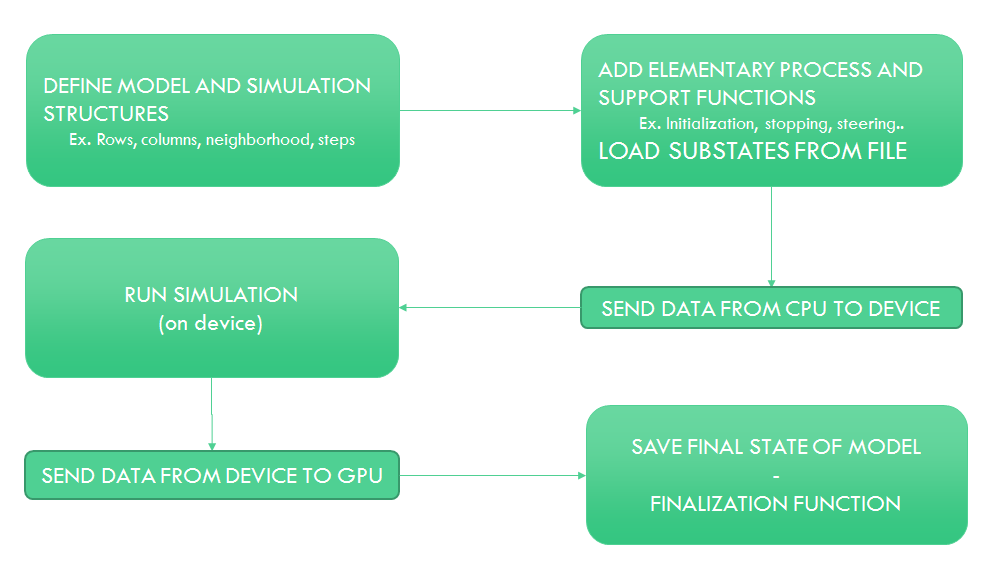
\includegraphics[width=1.0\columnwidth]{Immagini/opencalcudadiagram} 
\caption[Ciclo di vita del software OpenCAL-CUDA]{Diagramma del ciclo di vita
del software OpenCAL-CUDA}
\label{fig:opencalcudadiagram} 
\end{figure}

\section{Scelte progettuali}

In questo paragrafo si mostreranno le scelte progettuali e le pi� importanti
differenze implementative della versione sequenziale della libreria e della
versione parallelizzata in CUDA.

\subsection{\textsf{CALModel2D} e \textsf{CudaCALModel2D}}
Per poter utilizzare la potenza delle GPU, come descritto nei capitoli
\ref{cap:CUDA} e \ref{cap:Il calcolo parallelo}, � essenziale trasportare i dati
del programma sulla memoria del device. Il primo passo � stato appunto capire
come poter trasportare (\ref{par:datatrasfer}) la struct \textsf{CALModel2D} sul device.
All'inizio poteva sembrare semplice grazie alla funzione \textsf{cudaMemcpy\{
\ldots \}}, ma come vedremo non � stato possibile utilizzarla in questo caso, o
meglio, non � stato possibile lasciare l'incarico della copia
dell'oggetto al motore di CUDA. La presenza infatti di puntatori (e puntatori
di puntatori) all'interno di \textsf{CALModel2D} � stata la causa di tutto ci�.
Infatti, come ben sappiamo, la copia di un puntatore non � nient'altro che la
copia dell'indirizzo di memoria dove � allocato il puntatore, ed un oggetto sul
device non pu� avere all'interno puntatori allocati sulla memoria dell'host.
Dunque il primo passo � stato rendere pi� dettagliata
possibile la struct \textsf{CALModel2D}.
L'opzione adottata � stata scorporare le struct (e i puntatori a struct)
interne, come \textsf{CALCell2D} e \textsf{CALSubstate2D(b|i|r)}, rendendo il
loro contenuto parte della struct principale \textsf{CALModel2D}, in questo modo
si � perso un grado di astrazione ma rendendo vantaggioso il trasferimento dei
dati da device a host e viceversa.
Come si pu� notare nei codici \ref{lst:definitionModel2} e
\ref{lst:definitionModelCuda}, che mostrano le strutture \textsf{CALModel2D} e
\textsf{CudaCALModel2D}, si notano implementazioni in genere molto diverse ma
rappresentano un modello nella medesima maniera. Infatti l'utente non si render�
mai conto della differenza tra i due tipi di struttura.

\medskip
\lstinputlisting[caption={La rappresentazione del modello in OpenCAL.},
label=lst:definitionModel2, style=input]{code/CALModel2D.c}

Un esempio lampante � la rappresentazione dei sottostati.
\textsf{CALSubstate2D(b|i|r)} mentre in \textsf{CALModel2D} � rappresentato da
un puntatore a struct, in \textsf{CudaCALModel2D} � rappresentato da una coppia
di puntatori \textit{next} e \textit{current} per ogni tipo di sottostato.


\medskip
\lstinputlisting[caption={La rappresentazione del modello in OpenCAL-CUDA.},
label=lst:definitionModelCuda, style=input]{code/CudaCALModel2D.c}

Per il caso delle variabili scalari e per i processi elementari invece, il
codice � rimasto sostanzialmente uguale. 

Questa prima parte di studio ha evidenziato come la differenza di architettura e
il passaggio di dati tra la memoria device e host possano essere determinanti
sia in termini di performance che di sviluppo del progetto. Non � l'unico caso in
cui si � dovuto ricorrere ad un codice adattato per tradurre il codice
sequenziale in parallelo.

\subsection{\textsf{CALRun2D} e \textsf{CudaCALRun2D}}

Rispetto a \textsf{CALModel2D}, la struct \textsf{CALRun2D} ha subito meno
cambiamenti nella versione parallela della libreria, sia perch� c'erano meno
punti critici sia perch� la maggior parte dei cambiamenti sono dovuti ad
aggiunte di strutture dati. La loro implementazione � rappresentata dai codici
\ref{lst:definitionSimulation} e \ref{lst:definitionSimulationCuda}
rispettivamente per \textsf{CALRun2D} e \textsf{CudaCALRun2D}. 

Naturalmente nella versione parallela il modello � presente all'interno della
simulazione, cos� come accade per \textsf{CALRun2D}, e in particolare
troviamo tre diversi modelli.

Da premettere che, come descritto nel diagramma in fig.
\ref{fig:opencalcudadiagram} tutta la parte di simulazione avviene lato device.
Questo comporta dunque la presenza dei dati del modello sul device che
spiega la presenza dunque di un modello in pi� (\textsf{device\_ca2D}).
La presenza di \textsf{h\_device\_ca2D} invece � richiesta per le operazioni di
trasferimento dati tra l'host e il device. I dettagli implementativi relativi a
questa scelta progettuale verranno spiegati nel paragrafo successivo
(\ref{par:datatrasfer}).
Naturalmente \textsf{h\_device\_ca2D} non incide assolutamente sull'utilizzo di
OpenCAL, infatti l'utente non verr� mai a conoscenza della sua presenza poich� �
utilizzata solo nel core della libreria. Invece \textsf{device\_ca2D} comporta
una piccola modifica di utilizzo di OpenCAL ed � l'utente stesso che deve
dichiararla nel main principale e lasciare il compito della definizione alla
libreria aggiungendola come parametro alla funzione \textsf{calCudaRunDef2D}.

Vediamo insieme ora le due diverse implementazioni della struct dedicata alla
simulazione:

\medskip
\lstinputlisting[caption={La rappresentazione del modello in OpenCAL.},
label=lst:definitionSimulation, style=input]{code/CALRun2D.c}

\medskip
\lstinputlisting[caption={La rappresentazione del modello in OpenCAL-CUDA.},
label=lst:definitionSimulationCuda, style=input]{code/CudaCALRun2D.c}


\subsection{Trasferimento dei dati tra Host e Device}
\label{par:datatrasfer}
Il trasferimento dei dati utili alla computazione tra GPU e CPU � sempre stato
uno dei punti critici del parallelismo su dispositivi grafici. Perci� negli anni
le architetture hanno sviluppato diverse tecniche performanti per migliorare
questo aspetto. In CUDA C utilizzare le funzioni fornite dall'API �
molto conveniente perch� sono ottimizzate. La conferma la si pu� benissimo
trovare nel Visual Profiler (\ref{par:visualprofiler}) con dei semplici
toy-problems.

Nel caso di OpenCAL-CUDA il trasferimento dei dati � stato pi� complesso del
previsto. Come accennato in precedenza, le sole API di CUDA non sono bastate per
trasferire un modello tra la GPU e la CPU. Per questo � stato utilizzata una
procedura ad hoc per questo tipo di trasferimento.

Il problema principale del trasferimento dei dati da host a device � stato il
passaggio di strutture dati dichiarate tramite puntatori. In generale lato host
non si pu� accedere a blocchi di memoria su device e viceversa. Dunque copiare
l'indirizzo di un puntatore non era la scelta corretta. 

Per copiare un puntatore da host a device in CUDA bisogna copiare il
contenuto della struttura dati puntata, all'interno di una nuova struttura dati
allocata correttamente sul device. Il modello
\textsf{h\_device\_ca2D} dichiarato all'interno di \textsf{CudaCALRun2D} ha il
compito di fare da intermediario tra l'host e il device. Cio�, � un
\textit{oggetto} allocato sulla CPU ma con i puntatori a strutture
dati (vicinato, sottostati etc.) allocati sul device. Se vogliamo
copiare un modello di automa cellulare da host a device eseguiamo i seguenti passi:
\begin{enumerate}
  \item Allocare e definire (popolare) sull'host un oggetto
  \textsf{CudaCALModel2D} (chiamiamolo \textbf{host\_model})
  \item Allocare su device un oggetto \textsf{CudaCALModel2D} (chiamiamolo
  \textbf{device\_model})
  \item Allocare su host un oggetto \textsf{CudaCALModel2D} con i puntatori alle
  strutture dati allocati sul device (chiamiamolo \textbf{ibrid\_model})
  \item Copiare con una semplice \textsf{memcpy} le variabili scalari di
  host\_model su ibrid\_model.
  \item Copiare, utilizzando la funzione fornita dalle API di Cuda
  \textsf{cudaMemCpy}, il contenuto delle strutture dati (gestite tramite
  puntatori) di host\_model su ibrid\_model
  \item Copiare, utilizzando la funzione fornita dalle API di Cuda
  \textsf{cudaMemCpy}, tutto l'oggetto ibrid\_model su device\_model
\end{enumerate}

Il processo sembra senza dubbio tortuoso ma in realt� � un passo obbligato se si
vogliono utilizzare struct di questo genere. Il perch� del suo funzionamento �
semplice e lo insegnano gli errori di compilazione incontrati durante la fase
implementativa. 

Ad esempio se provassimo a copiare l'indice $i$ del
vicinato presente in \textsf{CudaCALModel2D} direttamente da host\_model a
device\_model ci si troverebbe davanti il seguente codice:

\medskip
\lstinputlisting[caption={},
label=lst:ipointercopy, style=input]{code/host_device.c}

Questo codice tuttavia risulta sbagliato poich� da host stiamo cercando di
accedere direttamente alla memoria sul device (\textsf{device\_model->i}) poich�
device\_model � allocato interamente su device. E' per questo che torna utile l'utilizzo
di una struttura intermedia accennata in precedenza (ibrid\_model).
Una copia corretta del codice \ref{lst:ipointercopy} potrebbe essere:

\medskip
\lstinputlisting[caption={},
label=lst:ipointercopy, style=input]{code/host_h_device.c}

In questo modo c'� la certezza che non si tenta di accedere sul device dal
codice compilato lato host e la copia va a buon fine. In particolare la seconda
copia va a buon fine poich� quando \textsf{cudaMemcpy} andr� a copiare l'intero
oggetto adesso pu� benissimo copiare l'indirizzo dei puntatori tra le due struct
poich� entrambi gli indirizzi sono allocati sul device.

Un esempio completo della copia del modello da host a device � mostrato nel
codice \ref{lst:copyhd}

\medskip
\lstinputlisting[caption={},
label=lst:copyhd, style=input]{code/copyhd.c}

Si pu� notare che il processo inverso (da device a host) � del tutto simile e
applica la seguente procedura al contrario:

\medskip
\lstinputlisting[caption={},
label=lst:copydh, style=input]{code/copydh.c}

L'oggetto \textit{copy\_model} presente nel codice sarebbe il nostro
ibrid\_model dichiarato nello stesso file. In particolare il metodo
\textsf{calCudaAllocatorModel} (cod. \ref{lst:copyhd})prende in input il modello
e ne copia gli scalari in copy\_model, allocando in seguito tutti i puntatori all'interno sul device in
modo da avere l'oggetto pronto alla nostra copia tra host e device.

In seguito si mostra il contenuto della funzione \textsf{calCudaAllocatorModel}:
\medskip
\lstinputlisting[caption={},
label=lst:allocatormodel, style=input]{code/allocatormodel.c}


\subsection{L'ottimizzazione delle celle attive}
\label{par:streamcompaction}
L'ottimizzazione � una keyword che si utilizza spesso quando si parla di
parallelismo e tecniche di performance. Gli automi cellulari hanno diverse
tecniche di ottimizzazione. 
Come ben sappiamo infatti alcuni di loro richiedono un tempo
computazionale elevato, ragion per cui, nel tempo, sono state ideate delle
tecniche di minimizzazione della complessit�. 

Una tecnica molto utilizzata e perfomante � la tecnica delle celle attive.
Una cella si dice attiva quando non si trova in uno stato ``quiescente" cio� ad
un determinato tempo $t$ la funzione di transizione cambia uno o pi� stati
della cella.

Un esempio banale potrebbe essere una colata lavica rappresentata da un automa cellulare. 
Uno degli stati di una cella potrebbe essere la quantit� di lava che deve ancora
\textit{colare}. 
Tutte le celle che contengono lava possono essere definite \textbf{celle
attive}.
Le funzioni di transizione spesso possono essere realmente complesse e richiedono
un elevato tempo computazionale. Grazie a questa tecnica di ottimizzazione
si pu� supporre che la funzione di transizione viene eseguita solamente
dalle celle in cui avviene un'evoluzione al tempo $t$ e nelle loro
vicine. 

Pensate bene che nel caso di una colata lavica una morfologia pu�
generare una matrice con migliaia di celle tra cui nei primi step della
computazione solo poche celle attive. Avviando la funzione di transizione solo
per le celle realmente attive si pu� guadagnare dunque tanto carico di lavoro.

Quello descritto � un approccio intuitivo e se entriamo nei dettagli
implementativi possiamo notare come questa ottimizzazione comporta l'aggiunta di
strutture dati a supporto. Una di queste, la pi� importante, � sicuramente la
matrice di \textsf{FLAGS}. Quest'ultima possiamo rappresentarla come una
matrice booleana in cui il valore \textsf{TRUE} nella posizione
\textit{i-esima} sta a significare che la cella � attiva, \textsf{FALSE}
altrimenti. Per poter accedere in scrittura alla matrice di flags in un
programma parallelo bisogna considerare l'utilizzo dell'esclusivit� in quanto
bisogna mantenere la lista di celle attive in uno stato coerente. In CUDA
l'esclusivit� � gestita dalle funzioni atomiche descritte nel capitolo
\ref{cap:CUDA}.

Capiamo bene che per stilare una lista delle celle in cui deve avvenire la
computazione allo step successivo bisogna obbligatoriamente scorrere la matrice
di flags e vedere quali sono attive e quali no. Scorrere tutta la matrice di
flags per� pu� diventare oneroso in termini di performance. Per questo esiste
un'altra tecnica subordinata chiamata \textbf{stream
compaction}\cite{STREAM:2009}.

\begin{figure}[H] 
\centering 
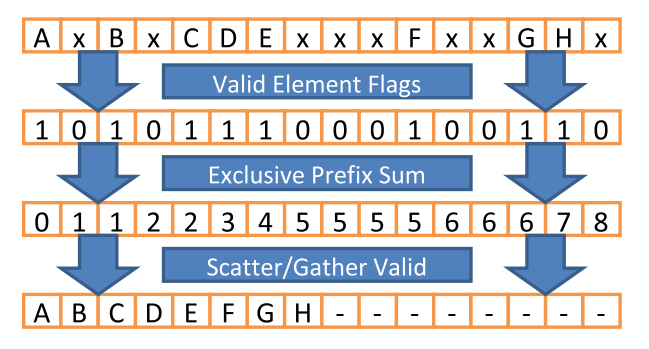
\includegraphics[width=0.75\columnwidth]{Immagini/streamc2} 
\caption[Esempio di stream compaction]{Esempio di stream compaction}
\label{fig:streamc} 
\end{figure}

Gli algoritmi di stream compaction attraverso semplici passaggi rimuovono
gli elementi non utili da un insieme di dati sparsi. Nel nostro caso, questo
genere di algoritmi, prendono in input la matrice di flags e restituiscono in
output un array con in testa le celle in cui il flag � ``true''. In
particolare, l'algoritmo si porta dietro l'indice delle celle attive poich�
identifica la posizione in cui andare a lanciare la funzione di transizione al
passo successivo.

In OpenCAL-CUDA � stata implementata tramite l'utilizzo della libreria
\textsf{chag} creata appunto dagli autori dell'articolo scientifico
``Efficient Stream Compaction" citato in precedenza \cite{STREAM:2009}
\cite{CHAG:2009}.

Inizialmente si era utilizzata la libreria \textbf{thrust} \cite{THR} ma dopo
una serie di test risultava inefficiente per il nostro tipo di problema e dunque � stata
scartata a favore della libreria chag::pp.

Mostriamo ora l'utilizzo dell'algoritmo di stream compaction all'interno della
libreria:

\medskip
\lstinputlisting[caption={Stream compaction in OpenCAL-CUDA},
label=lst:streamcompactioncuda, style=input]{code/streamc.c}

Seguendo step by step il codice si mostra come l'algoritmo viene utilizzato
solamente nel caso in cui l'utente abbia scelto di ottimizzare la simulazione
tramite la tecnica delle celle attive. Nel caso in cui le celle attive si
aggiornano viene avviato un kernel che ha il compito di aggiornare la lista di
flags trasformandoli in indici. Questo perch� all'algoritmo interessa quali sono
gli indici (in matrici lineari) delle celle attive in modo da sapere su quali
celle deve essere lanciata la funzione di transizione allo step successivo. La
funzione cruciale � \textsf{pp::compact\{\ldots\}} che prende in input:
\begin{enumerate}
  \item Il range di celle dell'array di indici sparsi (aggiornato dal kernel
 descritto in precedenza)
  \item L'array di output utile per ricavare le informazioni finali
  \item La dimensione dell'array
  \item Una funzione predicato
\end{enumerate}
La funzione predicato � definita da una struct eseguendo un
override dell'operatore (). Il predicato definisce la regola secondo cui
l'algoritmo deve compattare la matrice. Nel nostro caso se trova nell'array un
valore diverso da -1 lo inserisce al primo posto disponibile in testa,
altrimenti va avanti.

L'utilizzo di questa tecnica ha portato ad un guadagno del 30\% delle
performance.

\section{Struttura di OpenCAL-CUDA}
In questa sezione vedremo insieme come si utilizza in maniera completa la
libreria OpenCAL-CUDA.

\subsection{Il \textit{main}}
L'obiettivo principale di OpenCAL-CUDA era quello di fornire una versione di
OpenCAL completamente parallela mantenendo la stessa struttura, in modo da
rendere il parallelismo completamente trasparente all'utente. Nonostante ci�,
date alcune circostanze e la differenza di architetture, l'utilizzo della
libreria � leggermente cambiato in base all'esigenze dell'architettura CUDA.

Per poter utilizzare la libreria OpenCAL-CUDA possiamo stabilire i seguenti
passi:

\begin{itemize}
  \item Definizione e allocazione del modello e della simulazione
  \item Definizione e allocazione dei kernel e dei sottostati
  \item Trasferimento dei dati dall'host al device
  \item Definizione del ciclo di esecuzione
  \item Trasferimento dei dati dal device all'host
  \item Operazioni di finalizzazione
\end{itemize}

Come si pu� notare � presente qualche passo in pi� rispetto all'utilizzo della
versione sequenziale della libreria. Questo per consentire il passaggio di dati
tra le memorie poich� la simulazione avviene totalmente su GPU.

Come ricordato in precedenza, date alcune limitazioni nel passaggio di memoria
(\ref{par:datatrasfer}), si � perso un livello di astrazione rispetto ad
OpenCAL. Questo ha comportato dei leggeri cambiamenti anche in alcune funzioni
utilizzate nella libreria. Possiamo portare un esempio:

\textsf{calAddSubstate(b|i|r)} come mostrato nel capitolo \ref{cap:OpenCAL}
si implementava nel seguente modo:

\medskip
\lstinputlisting[caption={},
label=lst:addsubstates, style=input]{code/addsubstates.c}

In OpenCAL-CUDA l'implementazione cambia leggermente. Poich� i sottostati sono
rappresentati da matrici lineari (una per ogni tipo supportato, \textit{byte,
integer, real\ldots}), \textsf{calCudaAddSubstate} risulta leggermente diverso
rispetto alla sua versione sequenziale. Vediamone un esempio:

\medskip
\lstinputlisting[caption={},
label=lst:addsubstatescuda, style=input]{code/addsubstatescuda.c}

Con questa nuova versione la chiamata alla funzione � unica per ogni tipo di
dato. Dunque l'allocazione in memoria viene effettuata una sola volta per tutti
i sottostati di tipo uguale. La prima differenza sta nel fatto che l'utente deve
stabilire a priori il numero di sottostati per ogni tipo che desidera. Questo
non dovrebbe essere un grosso problema poich� si suppone che l'utente che decide
di utilizzare OpenCAL ha gi� bene in mente quale sia il suo modello e gi�
possiede queste informazioni. Nonostante ci� rimane libero di cambiare le sue
informazioni in qualsiasi momento. Una seconda differenza sta nelle funzioni di
\textit{load}. Siccome la nostra struttura dati � ora una matrice lineare, ogni
sottostato possiede un indice in modo tale da conoscere qual � il range di
memoria che occupa. Questo per facilit� pu� essere
rappresentato da un enumerativo che rende il codice abbastanza chiaro e lineare.

Per quanto riguarda invece le operazioni di trasferimento dei dati, sono gestite
automaticamente dalla libreria grazie a due funzioni:
\textsf{calInitializeInGPU2D} e \textsf{calSendDataGPUtoCPU}. Queste due
funzioni prendono in input il modello allocato sull'host e il modello allocato
sul device e rispettivamente trasferiscono i dati da CPU a GPU e viceversa.

Un'altra aggiunta naturalmente riguarda le funzioni relative alla simulazione
dell'automa cellulare. Mentre la definizione delle funzioni di inizializzazione
e supporto rimangono sostanzialmente uguali alla versione sequenziale, la
funzione \textsf{calRun2D} ha subito un leggero cambiamento. Come ben sappiamo
CUDA utilizza una serie di threads suddivisi in griglie e blocchi. In
OpenCAL-CUDA lasciamo al libert� all'utente di gestire questa configurazione a
patto che il core della libreria venga informata della scelta. Per questo due
valori di tipo \textsf{dim3} devono essere incluse tra gli input della funzione
\textsf{calCudaRun2D}.

Ecco un confronto tra la versione sequenziale e quella parallela:

\medskip
\lstinputlisting[caption={},
label=lst:calruncuda, style=input]{code/calruncuda.c}


\subsection{La dichiarazione dei \textit{kernel}}
I kernel per OpenCAL-CUDA sono tutte le funzioni che devono eseguire codice
parallelo. La libreria richiede che la funzione di inizializzazione,
la funzione di steering, la funzione di stop e i processi elementari devono
essere definite come kernel. Questo perch� sono le funzioni che verranno avviate
in parallelo dalla libreria attraverso l'architettura CUDA. 

Questa tipologia di funzioni sono dichiarate in maniera del tutto simile alla
versione sequenziale ma con l'aggiunta della keyword \textsf{\_\_global\_\_} che
identifica un kernel. All'interno di queste funzioni l'utente deve progettare
l'algoritmo parallelo a suo piacimento mettendo in pratica i concetti base di
CUDA. OpenCAL-CUDA fornisce delle comode funzioni per ricevere delle
informazioni molto utilizzate nei programmi scritti in CUDA C.
Ad esempio, capita spesso che un programmatore debba ricavarsi le informazioni
riguardo l'ID univoco dei threads. Questo comporta piccoli calcoli matematici
che a lungo andare possono diventare annoianti e ripetitivi,
inoltre ci si pu� imbattere in piccoli errori di calcolo. Per questo la libreria
OpenCAL-CUDA esegue tutte queste operazioni di routine in automatico tramite
alcune chiamate a funzione.

Mostriamo un esempio di processo elementare implementato tramite la libreria
OpenCAL-CUDA:

\medskip
\lstinputlisting[caption={},
label=lst:kernelcuda, style=input]{code/kernelcuda.c}


\section{Game of Life in OpenCAL-CUDA}
\label{par:gol-cuda}
Come descritto nel paragrafo \ref{par:gol} il Game of Life � il pi� famoso
automa cellulare. Per questo possiamo prenderlo da esempio per la sua semplicit� e la
sua chiarezza. 
Vediamone insieme una sua implementazione tramite la libreria OpenCAL-CUDA.

\medskip
\lstinputlisting[caption={},
label=lst:golcuda, style=input]{code/life2Dcuda.c}

Quello mostrato � il classico esempio di implementazione di un modello e una
simulazione in OpenCAL-CUDA.
All'inizio del programma troviamo tutte le informazioni relative alle strutture
dati, path dei file di configurazione e stampa, librerie incluse etc.

Da notare l'enumerativo \textsf{SUBSTATE\_NAME}, utile per
accedere alla matrice linearizzata dei sottostati (in questo caso di byte).
Prima della dichiarazione del main troviamo tutti i kernel utili ai fini della
simulazione. Questi sono implementati come delle normali funzioni con la
differenza che il codice viene eseguito in parallelo da migliaia di threads.
Una delle funzioni di supporto descritte nel paragrafo precedente �
\textsf{calCudaGetOffset} che ha il compito di restituire l'ID univoco per ogni
thread che accede al kernel corrente.
In questo caso sono state utilizzate altre due funzioni di supporto:
\textsf{calCudaGetIndexRow} e \textsf{calCudaGetIndexColumn}. Queste vengono
utilizzate per risalire ai pi� comuni indici $i$ e $j$ di una matrice a partire
dalla matrice linearizzata e dall'ID univoco del thread. Sono state implementate
poich� spesso ci si trova a dover gestire un determinato angolo di celle nella
loro evoluzione e l'utilizzo di indici pu� essere molto utile.

Un ultimo commento � relativo alla leggibilit� del codice che nonostante
l'utilizzo della GPGPU programming � rimasto molto chiaro e ridotto. Questo pu�
essere visto come un enorme potenzialit� della libreria che evita dunque la
pesantezza di leggibilit� del codice parallelo per GPU.

\section{``SCIARA-fv2'' in OpenCAL-CUDA}

Come specificato nel paragrafo \ref{par:SCIARA} � stato implementato un modello
pi� complesso a livello computazionale per eseguire diversi
stressing test esaminando l'effettiva validit� del lavoro di tesi.
SCIARA � un modello basato su automi cellulari complessi (CCA, \ref{par:CCA}) che descrive il fenomeno di una colata lavica
(Per ulteriori dettagli \cite{SCIARA:2001} \cite{SCIARA:2004} o
par. \ref{par:SCIARA}). 

Il tempo totale impiegato per implementare la versione parallelizzata in
OpenCAL-CUDA a partire dalla versione OpenCAL � sicuramente un fattore
determinante per la riuscita del lavoro di tesi. Se il tempo per elaborare una
versione parallela di un automa cellulare in OpenCAL-CUDA supera il tempo
 di implementazione dello stesso automa cellulare in CUDA C, allora utilizzare
 la libreria non comporterebbe nessun valore aggiuntivo. Nelle
 prove effettuate non � risultato cos�. In particolare � avvenuto il contrario:
 in poche ore, sia per SCIARA che per altri modelli di test, si � implementata
 una versione correttamente parallelizzata e performante. 
 L'immediatezza del passaggio alla GPGPU programming tramite la libreria
 OpenCAL-CUDA � dunque uno dei punti di forza della libreria stessa.

\medskip
\lstinputlisting[caption={},
label=lst:define-cuda, style=input]{code/define-sciara-cuda.cu}

La prima parte di codice riguarda principalmente la definizione di tutti i
valori numerici relativi al fenomeno naturale. Tra queste definizioni troviamo
anche la dimensione del modello, il numero e il nome dei sottostati. Da notare
che, come per Game of Life, gli enumerativi sono utilizzati solo per la
leggibilit� e per un implementazione pi� semplice del modello. 

\medskip
\lstinputlisting[caption={},
label=lst:elementaryprocesses-cuda, style=input]{code/elementary-sciara-cuda.cu}

Il cuore dell'implementazione riguarda la scrittura dei kernel e delle
funzioni device. In particolare i kernel rappresentano le funzioni elementari
dell'automa cellulare. Rispetto alla versione sequenziale mostrata al paragrafo
\ref{par:SCIARA} si notano molte differenze, cos� come accade per Game of Life
(\ref{par:gol-cuda}). 

I sottostati in OpenCAL vengono gestiti tramite la struttura
\textsf{CALSubstate2D(r|i|b)}, come spiegato nei paragrafi precedenti tutto ci�
in OpenCAL-CUDA non accade. Tutti i sottostati, per ogni tipo di dato, sono
rappresentati da un'unica struttura dati lineare. L'utilizzo di enumerativi,
che rappresentano dunque l'indice per ogni sottostato nella matrice
linearizzata, garantisce non solo la leggibilit� del codice ma favorisce la
comprensione per un eventuale manutenzione al codice. L'enumerativo riesce a
dare un'idea precisa del sottostato che viene chiamato in causa.

\medskip
\lstinputlisting[caption={Esempio di utilizzo degli enumerativi in
OpenCAL-CUDA con diversi sottostati}, label=lst:main-cuda,
style=input]{code/substate-cuda-sciara.cu}

Infine il \textit{main} in cui vengono definite tutte le configurazioni e le
propriet� dell'automa cellulare. Viene definito il modello tramite la funzione
\textsf{calCudaCADef2D} e avviata la simulazione tramite la funzione
\textsf{calCudaRun2D}.

\medskip
\lstinputlisting[caption={},
label=lst:main-cuda, style=input]{code/main-sciara-cuda.cu}






%% !TEX encoding = UTF-8
% !TEX TS-program = pdflatex
% !TEX root = ../Tesi.tex
% !TEX spellcheck = it-IT

%************************************************
\chapter{Lorem}
\label{cap:lorem}
%************************************************

Lorem ipsum dolor sit amet, consectetuer adipiscing elit. Ut purus elit, vestibulum ut, placerat ac, adipiscing vitae, felis. Curabitur dictum gravida mauris. Nam arcu libero, nonummy eget, consectetuer id, vulputate a, magna. Donec vehicula augue eu neque.

\section{Esempi}

\subsection{Tabelle}

\lipsum

\begin{table}[tb]
\caption[Un esempio di tabella mobile]{Un esempio di tabella mobile.}
\label{tab:esempio}
\centering
\begin{tabular}{cc}
\toprule
$p$ & $\lnot p$ \\ 
\midrule
V   & F \\ 
F   & V \\
\bottomrule 
\end{tabular}
\end{table}

La tabella~\vref{tab:esempio} fornisce un esempio di tabella mobile.

\lipsum[1-2]


\subsection{Figure}

\lipsum[2]

\begin{figure}[tb] 
\centering 
\includegraphics[width=0.5\columnwidth]{GalleriaStampe} 
\caption[Un esempio di figura mobile]{Un esempio di figura mobile (l'immagine, che riproduce la litografia \emph{Galleria di stampe}, di M.~Escher,\index{Escher, M.~C.} proviene da \url{http://www.mcescher.com/}).}
\label{fig:galleria} 
\end{figure}

La figura~\vref{fig:galleria} fornisce un esempio di figura mobile.

\lipsum[3]

\begin{figure}[tb]
\centering
\subfloat[Asia personas duo.]
{\includegraphics[width=.45\columnwidth]{Lorem}} \quad
\subfloat[Pan ma signo.]
{\label{fig:ipsum}%
\includegraphics[width=.45\columnwidth]{Ipsum}} \\
\subfloat[Methodicamente o uno.]
{\includegraphics[width=.45\columnwidth]{Dolor}} \quad
\subfloat[Titulo debitas.]
{\includegraphics[width=.45\columnwidth]{Sit}}
\caption[Tu duo titulo debitas latente]{Tu duo titulo debitas
latente.}
\label{fig:esempio}
\end{figure}

La figura~\vref{fig:esempio} costituisce un esempio di figura mobile.

\lipsum[4]

%% !TEX encoding = UTF-8
% !TEX TS-program = pdflatex
% !TEX root = ../Tesi.tex
% !TEX spellcheck = it-IT

%************************************************
\chapter{Ipsum}
\label{cap:ipsum}
%************************************************


Lorem ipsum dolor sit amet, consectetuer adipiscing elit. Nam dui ligula, fringilla a, euismod sodales, sollicitudin vel, wisi. Morbi auctor lorem non justo. Nam lacus libero, pretium at, lobortis vitae, ultricies et, tellus.
\begin{description}
\item[Lorem ipsum dolor] sit amet, consectetuer adipiscing elit. Ut purus elit, vestibulum ut, placerat ac $\lim_{n \to \infty}\sum_{k=1}^n \frac{1}{k^2}= \frac{\pi^2}{6}$.
\item[Mauris ut leo.]
Cras viverra metus rhoncus sem. Nulla et lectus vestibulum urna fringilla ultrices. Phasellus eu tellus sit amet tortor gravida placerat.
\[
\lim_{n \to \infty}\sum_{k=1}^n \frac{1}{k^2}= \frac{\pi^2}{6}.
\]
\end{description}

Nulla malesuada porttitor diam. Donec felis erat, congue non, volutpat at, tincidunt tristique, libero. Vivamus viverra fermentum felis.
\begin{equation}
\label{eq:euler}
e^{i\pi}+1=0.
\end{equation}
Dalla formula~\eqref{eq:euler} 
si deduce che\dots






\section{Nozioni basilari}

\subsection{Insiemi numerici}

Donec nonummy pellentesque ante. Phasellus adipiscing semper elit.
\begin{equation}
x^2 \geq 0 \quad
\forall x \in \mathbb{R}.
\end{equation}


\subsection{Le matrici}

\lipsum[2]
\begin{equation}
A=
\begin{bmatrix}
x_{11} & x_{12} & \dots \\
x_{21} & x_{22} & \dots \\
\vdots & \vdots & \ddots
\end{bmatrix}
\end{equation}



\section{Formule fuori corpo}

Proin fermentum massa ac quam. Sed diam turpis, molestie vitae, placerat a, molestie nec, leo. Maecenas lacinia. Nam ipsum ligula, eleifend at, accumsan nec, suscipit a, ipsum. 


\subsection{Una formula spezzata con allineamento}

\lipsum[2]
\begin{equation} 
\begin{split} 
a &= b+c-d \\ 
  &= e-f \\ 
  &= g+h \\ 
  &= i. 
\end{split} 
\end{equation}

 
\subsection{Casi}

\lipsum[3]
\begin{equation}
f(n):=
\begin{cases} 
2n+1, & \text{con $n$ dispari,} \\ 
n/2,  & \text{con $n$ pari.} 
\end{cases} 
\end{equation}



\section{Enunciati e dimostrazioni}

Nunc eleifend consequat lorem. Sed lacinia nulla vitae enim. Pellentesque tincidunt purus vel magna. Integer non enim. Praesent euismod nunc eu purus.
\begin{definizione}[di Gauss] 
Un \emph{matematico} trova ovvio che
$\int_{-\infty}^{+\infty}
e^{-x^2}\,dx=\sqrt{\pi}$. 
\end{definizione} 
\begin{teorema} 
I matematici, se ce ne sono, sono molto rari.
\end{teorema} 

\lipsum[2]

\begin{teorema}[di Pitagora]
La somma dei quadrati costruiti sui cateti uguaglia il quadrato costruito sull'ipotenusa.
\end{teorema}
La dimostrazione viene lasciata per esercizio.

Donec bibendum quam in tellus. Nullam cursus pulvinar lectus. Donec et mi. Nam vulputate metus eu enim. Vestibulum pellentesque felis eu massa.
\begin{teorema}[Sorpresa]
Si ha che $\log(-1)^2=2\log(-1)$.
\end{teorema} 
\begin{proof} 
Si ha che $\log(1)^2 = 2\log(1)$.
Ma si ha anche che $\log(-1)^2=\log(1)=0$.
Quindi $2\log(-1)=0$, da cui la tesi.
\end{proof}
Viene un quadratino a fine dimostrazione.
\begin{legge}
\label{lex:capo}
Il capo ha ragione.
\end{legge}
\begin{decreto}[Aggiornamento alla legge~\ref{lex:capo}]
Il capo ha \emph{sempre} ragione.
\end{decreto}
\begin{legge}
Se il capo ha torto, vedere la 
legge~\ref{lex:capo}.
\end{legge}


Nam dui ligula, fringilla a, euismod sodales, sollicitudin vel, wisi. Morbi auctor lorem non justo. Nam lacus libero, pretium at, lobortis vitae, ultricies et, tellus.
\begin{murphy}
Cras nec ante. Pellentesque a nulla. Cum sociis natoque penatibus et magnis dis parturient montes, nascetur ridiculus mus. Aliquam tincidunt urna.
\end{murphy}

%\appendix
%% !TEX encoding = UTF-8
% !TEX TS-program = pdflatex
% !TEX root = ../Tesi.tex
% !TEX spellcheck = it-IT

%************************************************
\chapter{Dolor}
\label{cap:dolor}
%************************************************

\lipsum[1]

\section{Mane}
\lipsum[2]

\section{Tekel}
\lipsum[3]

\section{Fares}
\lipsum[4-5]




% *****************************************************************
% Materiale finale
%******************************************************************

% !TEX encoding = UTF-8
% !TEX TS-program = pdflatex
% !TEX root = ../Tesi.tex
% !TEX spellcheck = it-IT

%************************************************
\chapter{Conclusioni}
\label{cap:Conclusioni}
%************************************************

Gi� da molto tempo l'approccio sistematico al parallel computing ha comportato
miglioramenti generali nell'utilizzo dei sistemi informatici. La ricerca basata
sull'incremento delle performance dei moderni computer e il calcolo ad alte
prestazioni ha trovato campo fertile in numerosi settori dell'informatica tra i
quali la modellistica e la simulazione.

L'obiettivo di questo lavoro di tesi � stata la parallelizzazione della libreria
per lo sviluppo di modelli basati su automi cellulari OpenCAL. Gli automi
cellulari per loro natura si prestano egregiamente ad un approccio parallelo,
proprio per questo � stata immediata la scelta del parallel computing per
migliorare le performance della libreria OpenCAL. La versione parallela
OpenCAL-CUDA, come si intuisce, � stata implementata tramite l'archiettura CUDA
sviluppata e rilasciata dalla societ� NVIDIA Corporation. In particolare � stato
utilizzato il linguaggio CUDA C, estensione del linguaggio C, per
l'implementazione del codice parallelo.

Tutte le caratteristiche appartenenti ad OpenCAL sono state mantenute, tuttavia 
l'implementazione dei modelli e dei loro processi elementari sono state
adattate al tipo di architettura utilizzata. In particolare sono presenti alcuni
cambiamenti dovuti ad una filosofia implementativa diversa tra l'approccio
sequenziale e quello parallelo.

NVIDIA dal 2006 ai giorni nostri, ha rilasciato in maniera
frequente aggiornamenti per l'architettura CUDA con numerosi
miglioramenti relativi alla leggibilit� del codice e alle performance. Le API di
CUDA compatibili con i device NVIDIA hanno consentito la realizzazione
del progetto.

Gli automi cellulari, come spiegato nel capitolo \ref{cap:Automi Cellulari},
evolvono basandosi sulla funzione di transizione, in particolare per gli automi
cellulari complessi (CCA, \ref{par:CCA}) l'evoluzione dipende da pi� processi
elementari. Questa funzione di transizione viene eseguita allo stesso modo su
ogni cella dello spazio cellulare. Questo tipo di approccio viaggia in
perfetta sintonia con la filosofia del parallel computing.

In OpenCAL-CUDA vengono creati un numero di blocchi e thread in base al numero
di celle dello spazio cellulare in modo tale da assegnare un thread per ogni
cella. In questo modo, tutti i thread eseguono la stessa operazione nello stesso
momento su celle diverse incrementando le performance e minimizzando i tempi di
risposta. Per l'implementazione di un automa cellulare si pu� utilizzare anche
l'ottimizzazione delle celle attive. Questo approccio, che utilizza solamente le
celle attive escludendo le celle in stato quiescente, � supportato dalla
versione parallela grazie all'utilizzo della stream compaction (par.
\ref{par:streamcompaction}). La stream compaction ha il compito di elaborare e
comprimere i dati sparsi. I dati sparsi nel nostro caso sono il numero di celle
attive ad un determinato tempo $t$. Si istanzieranno dunque un determinato
numero di thread in base al numero di celle effettivamente attive.

Dopo aver terminato la parallelizzazione di OpenCAL sono stati implementati
diversi modelli con il fine di testare il lavoro di tesi. Tra i vari modelli
implementati, quello utilizzato per confrontare i tempi di esecuzione e i vari
miglioramenti di performance � stato SCIARA \cite{SCIARA:2001}
\cite{SCIARA:2004}.
I test eseguiti si sono basati sull'implementazione del modello SCIARA sia con
l'ottimizzazione delle celle attive che senza alcun tipo di ottimizzazione. 

Per raccogliere i dati relativi ai tempi di esecuzione per la versione parallela
del modello � stata utilizzata la super-macchina ``Stromboli'' situata al centro
di calcolo ad alte prestazioni dell'Unical, dotata di un processore Quad Xeon da
2.8GHz. Per quanto riguarda le schede grafiche utilizzate sono state scelte due
differenti schede: la prima � una Tesla K20c, la seconda una GeForce GT750M
entrambe di marca NVIDIA.

Con OpenCAL-CUDA per la versione implementata senza ottimizzazioni raggiunge
una speedup di circa $29\times$ in media, utilizzando la scheda Tesla K20c. Per
quanto riguarda i test sulla versione con l'ottimizzazione delle celle attive
con 200 crateri raggiunge una speedup di circa $10\times$ utilizzando la scheda
GeForce GT 750M.

Oggi OpenCAL � un progetto open source avviato. Sono presenti anche diverse
implementazioni della libreria tra cui due versioni parallelizzate utilizzando
i linguaggi di programmazione OpenCL e OpenMP. Un ulteriore versione della
libreria integra OpenGL per la visualizzazione grafica. 

Un possibile sviluppo futuro di OpenCAL-CUDA potrebbe essere l'implementazione
della versione 3D, mentre a scopo statistico e di ricerca sarebbe sicuramente
interessante effettuare un confronto delle performance tra le varie
implementazioni parallelizzate.

% !TEX encoding = UTF-8
% !TEX TS-program = pdflatex
% !TEX root = ../Tesi.tex
% !TEX spellcheck = it-IT

%*******************************************************
% Ringraziamenti
%*******************************************************
\cleardoublepage
\phantomsection
\pdfbookmark{Ringraziamenti}{ringraziamenti}



\bigskip

\begingroup
\let\clearpage\relax
\let\cleardoublepage\relax
\let\cleardoublepage\relax

\chapter*{Ringraziamenti}
Un ringraziamento particolare lo devo a mio padre e mia madre che in tutti gli
anni universitari mi hanno sostenuto. Insieme ai miei fratelli, mi hanno
stimolato allo studio ed educato alla cultura: il miglior regalo ricevuto.
Ringrazio Eleonora per aver appoggiato le mie scelte durante gli ultimi anni
universitari e per avermi sempre spronato per raggiungere i miei obiettivi.

Un ringraziamento doveroso lo devo ai professori William Spataro e Donato
D'Ambrosio che mi hanno seguito con costanza, fornendomi consigli preziosi per
il mio lavoro di tesi. Inoltre ringrazio il dott. Davide Spataro, il
dott. Maurizio Macr� e il dott. Alessio De Rango per il loro supporto durante
questi ultimi mesi.

Un ultimo ringraziamento va all'Akademia Gorniczo-Hutnicza - University of
Science and Technology di Cracovia e al prof. Jaroslaw Was. Grazie alla loro
accoglienza e disponibilit� hanno reso indimenticabili i miei mesi di studio in
Polonia.




\bigskip


\endgroup



\listoffigures
\addcontentsline{toc}{chapter}{Lista delle figure}

\listoftables
\addcontentsline{toc}{chapter}{Lista delle tabelle}

\printbibliography
\addcontentsline{toc}{chapter}{\refname}

\end{document}
